\chapter{More on Virtual Memory}

\section{Page swapping}

A process can be swapped temporarily out of memory to HD and then brought back into memory for continued execution. The total logical memory space of processes can exceed physical memory.

\paragraph{HD} - fast disk large enough to accommodate copies of all
memory images for all users; must provide direct access to these
memory images.

\paragraph{Roll out, roll in} - swapping variant used for priority-based scheduling
algorithms; lower-priority process is swapped out so higher-priority
process can be loaded and executed.

\paragraph{}

Major part of swap time is transfer time; total transfer time is directly
proportional to the amount of memory swapped. System maintains a \textbf{ready queue} of ready-to-run processes which
have memory images on disk.

\paragraph{}
Does the swapped out process need to swap back in to same physical
addresses?

Usually not, but depends on address binding method, plus consider pending I/O to / from process memory space.

\paragraph{}

Each OS can decide how to manage the swap method:

\begin{itemize}
    \item Swapping normally disabled
    \item Started if more than threshold amount of memory allocated
    \item Disabled again once memory demand reduced below threshold
\end{itemize}

\begin{figure}[h!]
    \centering
    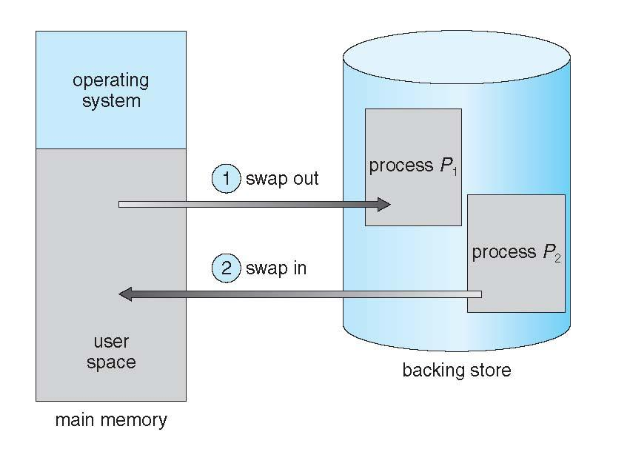
\includegraphics[width=0.5\linewidth]{img/dfbngt.png}
    \caption{Swapping process}
\end{figure}


\newpage
\subsection{Context Switch Time including Swapping}

If next processes to be put on CPU is not in memory and RAM is full,
you need to swap out a process and swap in target process. The context switch time can then be very high i.e. latency for getting data to HD.

\paragraph{Example: } 100MB process swapping to hard disk with transfer rate of 50MB/sec:

\begin{itemize}
    \item[] Swap out time of 2 seconds
    \item[] Plus swap in of same sized process
    \item[] Total context switch swapping component time of 4 s
\end{itemize}

Can reduce if reduce size of memory swapped – by knowing how
much memory really being used. System calls to inform OS of memory use via
\verb|request_memory()| and \verb|release_memory()|.

\paragraph{Other constraints: } if a task is pending I/O can’t swap out as I/O would occur to wrong process, or always transfer I/O to kernel space, then to I/O device but this cause  as double buffering, adds overhead.


So how does it work in \textbf{modern operating systems}?


\begin{itemize}
    \item[] Swap only when free memory is extremely low
    \item[] When using memory pages, entire pages are swapped in and out
    \item[] Swapped out pages are usually stored in a “paging file”
\end{itemize}

\begin{figure}[h!]
    \centering
    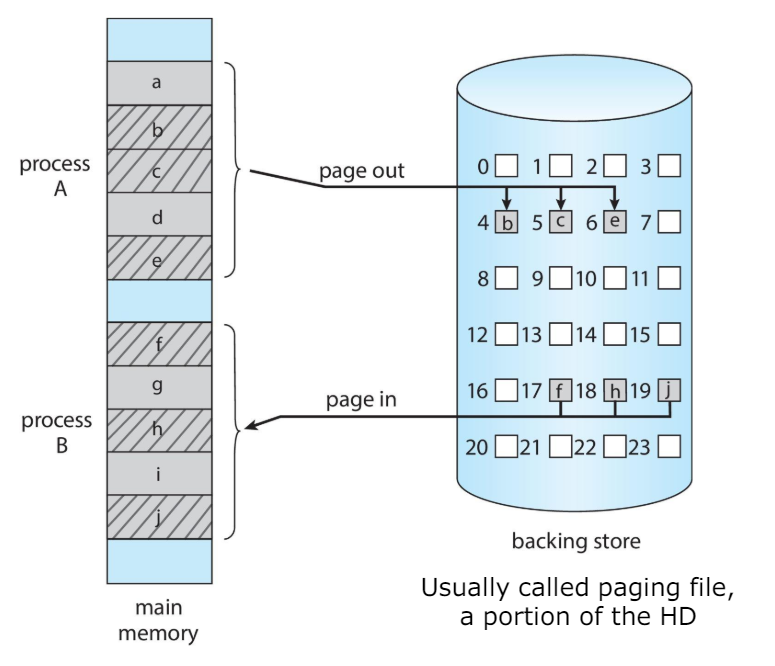
\includegraphics[width=0.7\linewidth]{img/ndgf.png}
    \caption{Swapping with Paging}
\end{figure}

\newpage
\subsection{Swapping on Mobile Systems}

The swapping is not typically used because the storage is small, the flash drive has limited number of write cycles and the bus between the flash memory and the CPU is limited.

So instead of using swapping when the free memory is low:

\begin{itemize}
    \item \textbf{iOS} asks apps to voluntarily relinquish allocated memory, Read-only data thrown out and reloaded from flash if needed. Failure to free can result in termination.
    \item \textbf{Android} terminates apps if low free memory, but first writes application state to flash for fast restart.
\end{itemize}


Both OSes support paging as discussed below.


\section{Structure of the Page Table}

Memory structures for paging can get huge using straight-forward methods. Consider a 32-bit logic address space, page size of 4KB, the page would have 1 million entry the total space for EACH process is 4MB only for get the physical address
space.

One simple solution is to divide the page table into smaller units, and loading it only partially: 

\begin{enumerate}
    \item Hierarchical Paging
    \item Hashed Page Tables
    \item Inverted Page Tables
\end{enumerate}


\subsection{Hierarchical Page Tables}

In this methods we break up the logical address space into multiple page tables. A simple technique is a two-level page table, in this way we load only the section we are interested in.

\begin{figure}[h!]
    \centering
    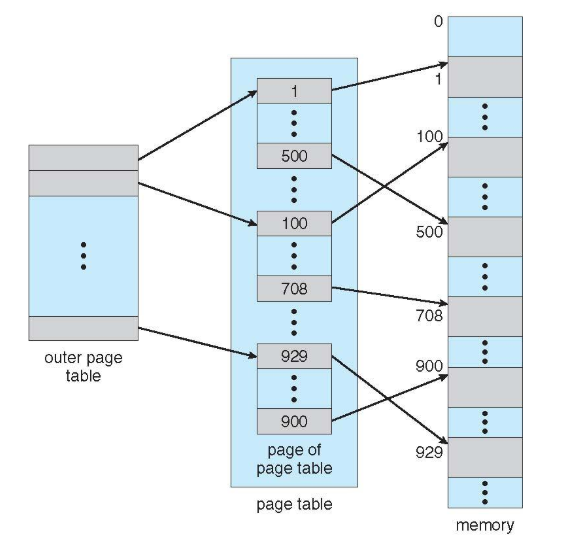
\includegraphics[width=0.6\linewidth]{img/sbdf.png}
\end{figure}

Now the 32-bit with 4K page size, is divides into:

\begin{itemize}
    \item a page number consisting of 20 bits is divided in two piece of 10-bit each:
    \begin{itemize}
        \item[] p1 to access the page of page tables, the \textbf{outer page}
        \item[] p2 to access the specific row of the “chunk” of page table, the \textbf{inner page}
    \end{itemize}
    \item a page offset consisting of 12 bits
\end{itemize}

\begin{figure}[h!]
    \centering
    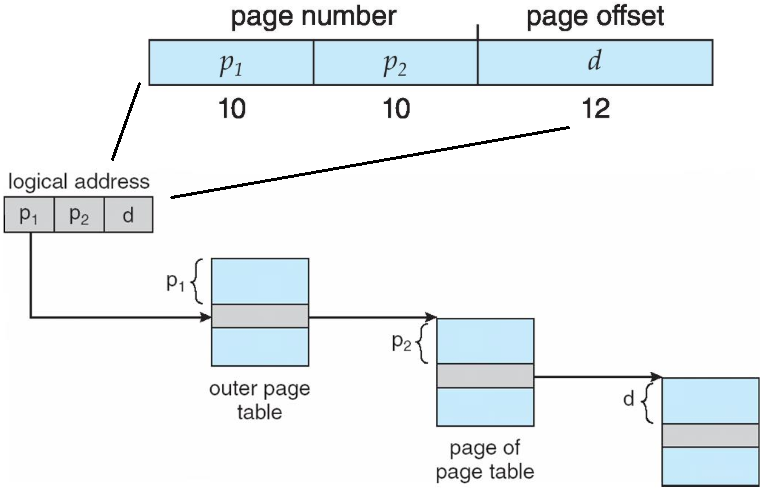
\includegraphics[width=0.65\linewidth]{img/mu.png}
\end{figure}


\subsubsection{64-bit Logical Address Space}

Even two-level paging scheme may not be sufficient, if page size is still 4 KB the page table has $2^{52}$ entries, the inner page tables could be $2^{10}$:

\begin{figure}[h!]
    \centering
    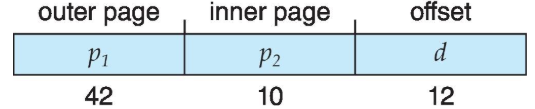
\includegraphics[width=0.5\linewidth]{img/ndg.png}
\end{figure}

The outer page table has $2^{42}$ entries witch is 4 terabytes per process! One solution could be add another layer of outer page table:

\begin{figure}[h!]
    \centering
    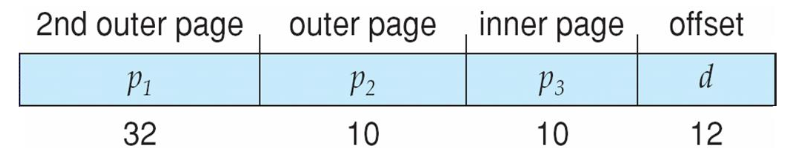
\includegraphics[width=0.65\linewidth]{img/db.png}
\end{figure}

The problem here is the 4 memory access to get one physical memory location, this is not a brilliant idea.

\newpage
\subsection{Hashed Page Tables}
Common address spaces is $> 32$-bit. The virtual page number is hashed into a page table, this page table contains a list of elements hashed to the same location.

Each elements contains:

\begin{itemize}
    \item the virtual page number
    \item the value of the mapped page frame
    \item a pointer to the next element
\end{itemize}

If you have and address space of 64-bit, 12 are offset, so 52 for page address. You can use an hash table of 4Kb ($2^{12}$), which typically fits in a single page and always stays in memory for each process. 

Then go to the specific page through it. If all the memory is used by the process, this is not efficient. However, in the vast majority of cases no process will fully use all $2^{52}$ pages.


\begin{figure}[h!]
    \centering
    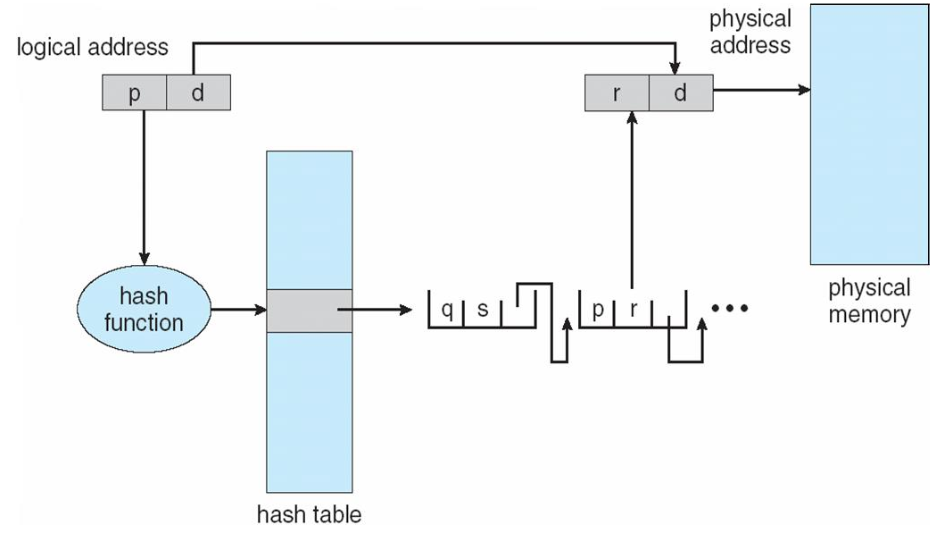
\includegraphics[width=0.75\linewidth]{img/ngf.png}
    \caption{Hashed Page Table}
\end{figure}

\subsection{Inverted Page Table}

Rather than each process having a page table and keeping track of all
possible logical pages, one entry for each real page of memory!

Each entry consists of the virtual address of the page stored in that real
memory location, with information about the process that owns that
page

\begin{figure}[h!]
    \centering
    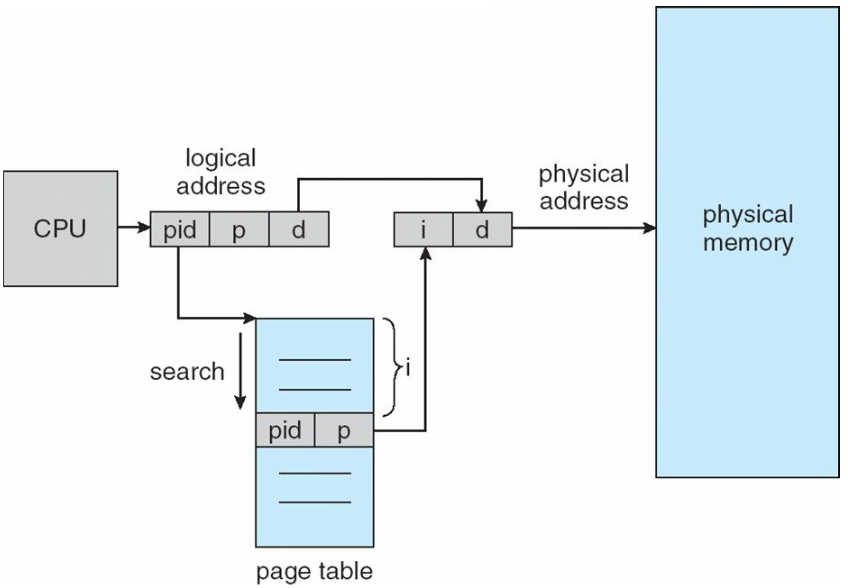
\includegraphics[width=0.65\linewidth]{img/sfb.png}
\end{figure}

Decreases memory needed to store each page table, but increases
time needed to search the table when a page reference occurs. 

One solution could be using hashing to limit the search to one, also TLB can accelerate access.
\newpage
\section{Segmentation}
Using pages of fixed sizes opens the problem of internal fragmentation, each process is matched to a given amount of pages rather than
memory it needs.

So, is there a way to assign exactly the amount of memory a process needs, thus avoiding any kind of memory waste? The answer is using \textbf{segmentation}.

\begin{figure}[h!]
    \centering
    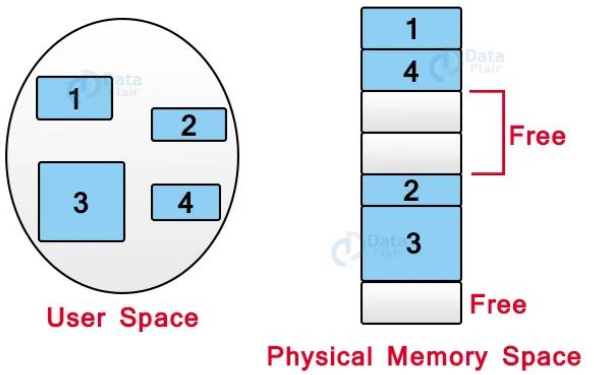
\includegraphics[width=0.5\linewidth]{img/sdavg.png}
\end{figure}

A process is divided into chunks, the chunks that a program is divided into, which are not necessarily all
of the exact sizes, are called segments. 

\begin{itemize}
    \item[--] A chunk for stack
    \item[--] A chunk for heap
    \item[--] A chunk for library 1
\end{itemize}

Each process is divided into several segments, all of which are loaded
into memory at run time, though not necessarily contiguously. 

A table stores the information about all such segments: the base and the limit (length).

\begin{figure}[h!]
    \centering
    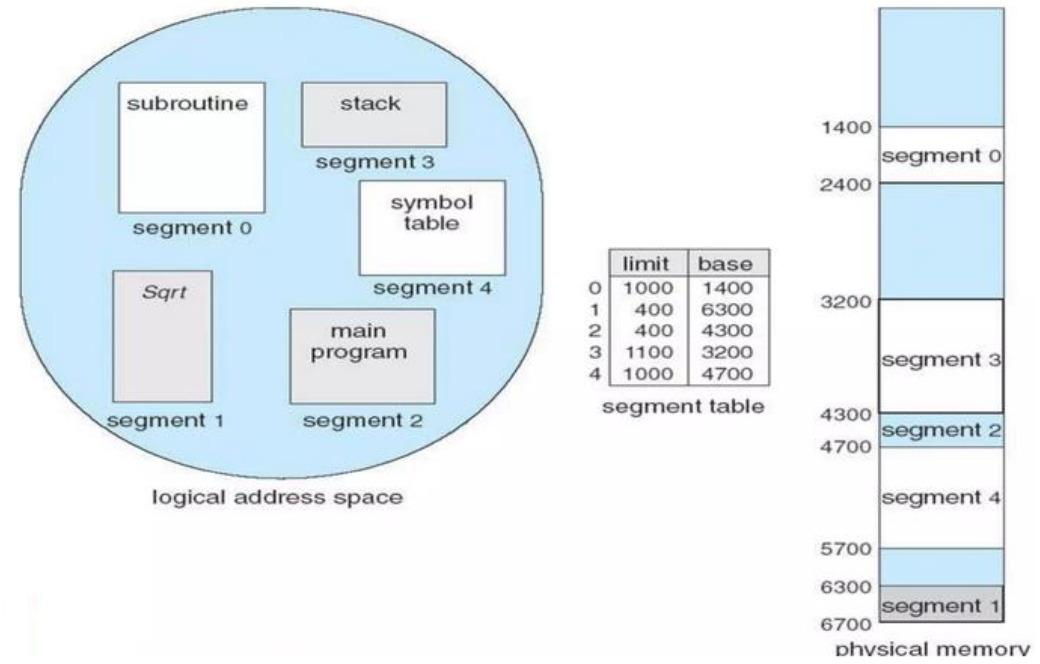
\includegraphics[width=0.75\linewidth]{img/dgn.png}
\end{figure}

\begin{figure}[h!]
    \centering
    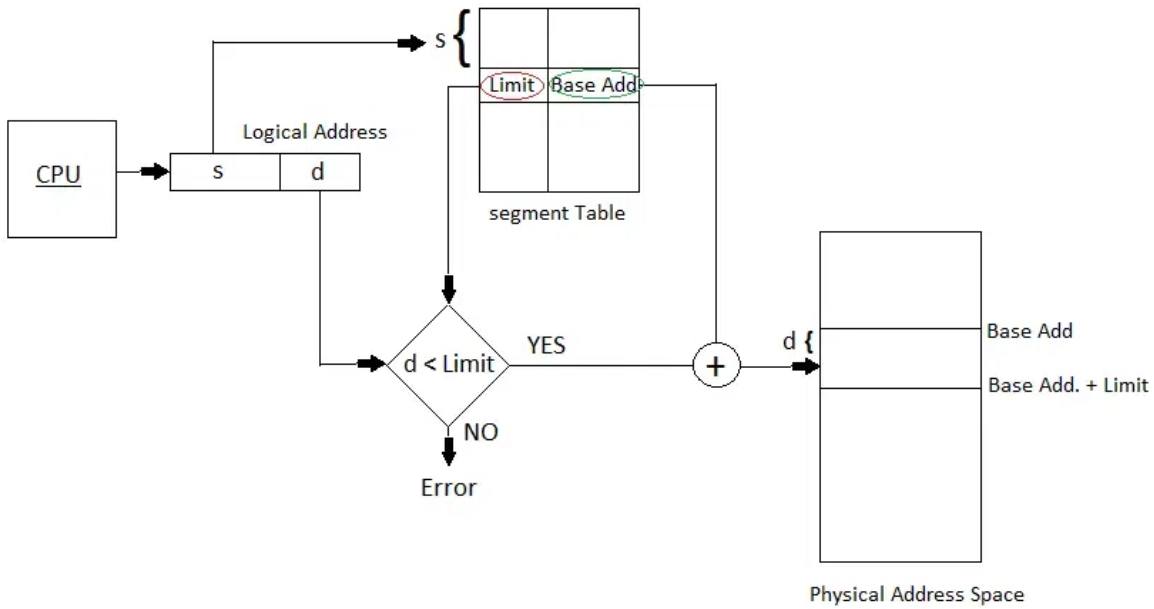
\includegraphics[width=0.75\linewidth]{img/dasv.png}
    \caption{Segmentation: logical to physical}
\end{figure}

\newpage
\subsection{Paging vs Segmentation}

\begin{figure}[h!]
    \centering
    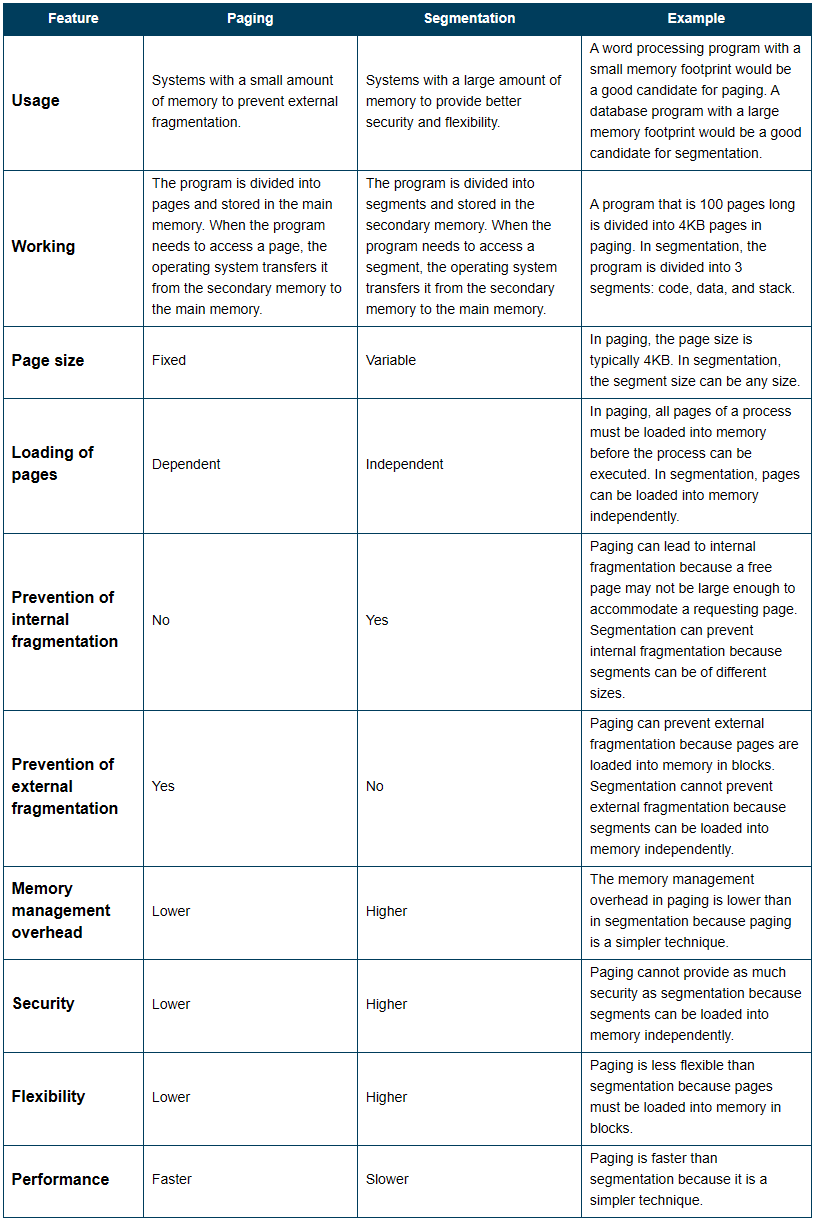
\includegraphics[width=1\linewidth]{img/dsfb.png}
\end{figure}

\newpage
\begin{figure}[h!]
    \centering
    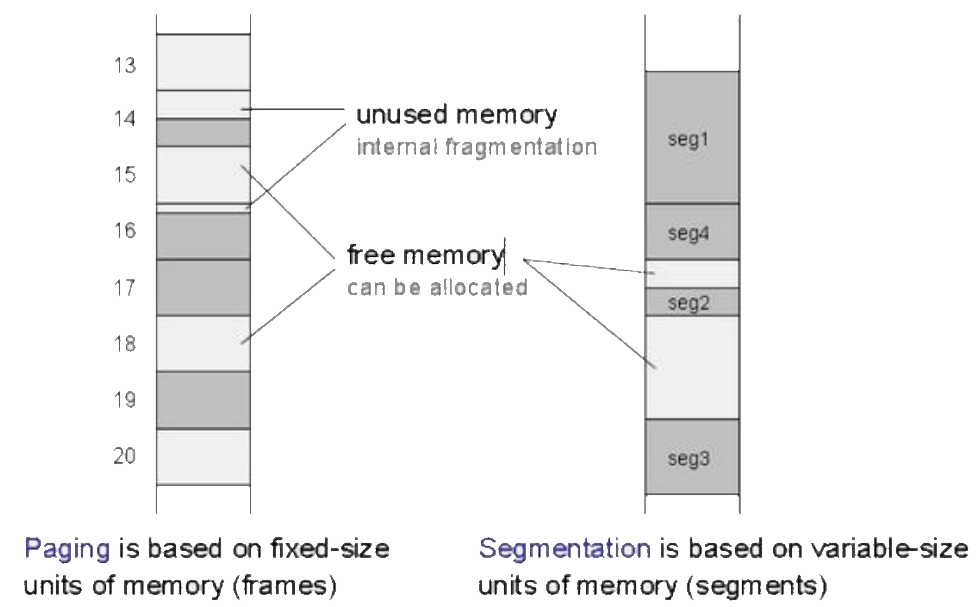
\includegraphics[width=0.75\linewidth]{img/Immagine 2024-05-22 170639.png}
\end{figure}

\subsubsection{Example of Intel IA-32 Architecture}

\begin{figure}[h!]
    \centering
    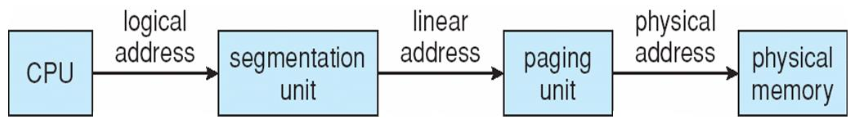
\includegraphics[width=0.65\linewidth]{img/dddbv.png}
    \caption{Memory address conversion}
\end{figure}

Paging units form equivalent of MMU, pages sizes can be 4 KB or 4 MB, two-level page tables.

\begin{figure}[h!]
    \centering
    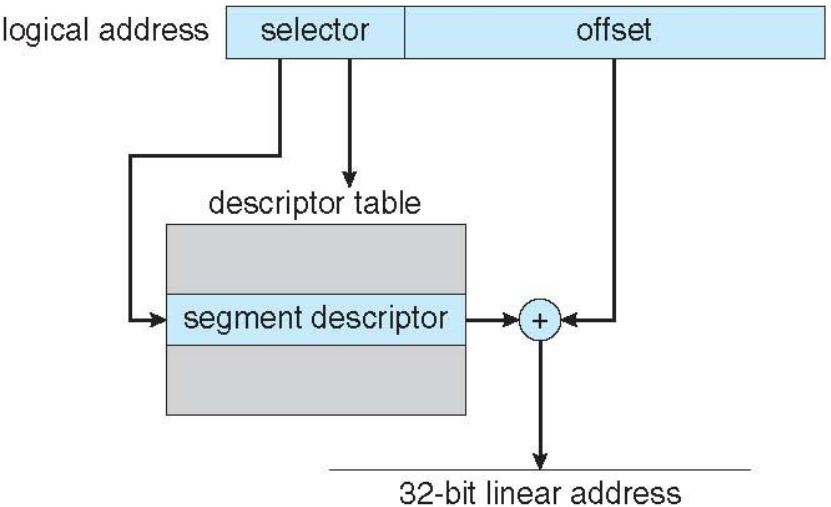
\includegraphics[width=0.55\linewidth]{img/abdv.png}
\end{figure}


\subsubsection{Example of Intel Intel x86-64}

Current generation of CISC architecture has 64 bits, this is ginormous  (> 16 exabytes). In practice only implement 48 bit addressing.

\begin{figure}[h!]
    \centering
    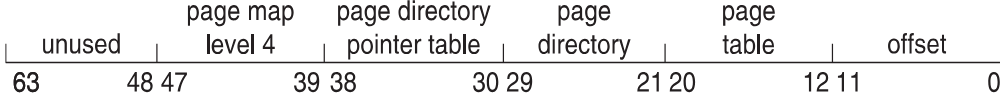
\includegraphics[width=0.9\linewidth]{img/fmhh.png}
\end{figure}


\chapter{Mass-Storage Systems}

Bulk of secondary storage for modern computers is \textbf{ hard disk drives}, HDD, and \textbf{nonvolatile memory}, NVM, devices.

\paragraph{HDDs} spin platters of magnetically-coated material under moving
read-write heads:


\begin{itemize}
    \item Drives rotate at 60 to 250 times per second
    \item Transfer rate is rate at which data flow between drive and computer, $\approx\,1$ Gb/sec
    \item Positioning time (random-access time) is time to move disk arm to desired cylinder (seek time) and time for desired sector to rotate under the disk head (rotational latency), from 3ms to 12ms
    \item Head crash results from disk head making contact with the disk surface -- That’s bad
\end{itemize}

\begin{figure}[h!]
    \centering
    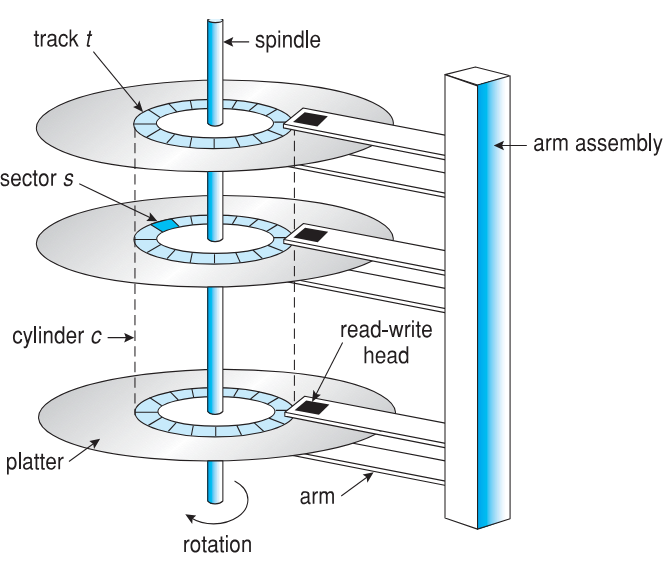
\includegraphics[width=0.75\linewidth]{img/yys.png}
\end{figure}


\begin{equation*}
    \text{Access Latency (Average access time) = average seek time + average latency}
\end{equation*}

For fastest disk: 3 ms + 2 ms = 5 ms.

\begin{equation*}
    \text{Average I/O time = average access time + (amount to transfer / transfer rate) + controller overhead}
\end{equation*}

\paragraph{Esample: }o transfer a 4KB block on a 7200 RPM disk with a 5ms
average seek time, 1Gb/sec transfer rate with a .1ms controller
overhead.

\paragraph{}
At 7200 RPM = 120 rev/sec = 8.333ms/rev, in the worst case, we have to wait 1 full revolution, but on average we have to wait a half-revolution or 4.17ms.


Transfer time = 4KB / 1Gb/s * 8Gb / GB * 1GB / 10242KB = 32 / ($1024^2$) = 0.031 ms

Average I/O time for 4KB block = 5ms + 4.17ms + 0.1ms + .031ms = 9.301ms

\section{Nonvolatile Memory Devices}

The NVM is intendef for the solid-state drives and the USB drive. This device are more reliable and \textbf{faster} than HDD but more expensive.

Read and written in “page” increments (think sector) but can’t
overwrite in place, must first be erased, and erases happen in larger ”block”
increments. This device can be erased a limit number of times called \textbf{drive writes per day}, DWPD.

\paragraph{}
The SSD is a complex device, it mount processor to look if all sector is in good conditions, erase and write block ecc.

\section{HD Scheduling}

The operating system is responsible for using hardware efficiently, for the disk this means having a fast access time and disk
bandwidth. The \textbf{bandwidth} is the total number of bytes transferred, divided by
the total time between the first request for service and the completion
of the last transfer.

\paragraph{}

There are many sources of disk I/O request: OS, System processes, Users processes; all includes write/read, disk address,
memory address, number of sectors to transfer. The OS maintains a queue of request per device.

In the past the HD is not sophisticated like now, before the OS must take care of all of thinks: queue management and disk
drive head scheduling. Now the control is up to the HD, the OS must pass only the block addresses and sorting the request.

\paragraph{Esample: } we want to manage the following list of request using different scheduling algorithm:

\begin{itemize}
\centering
    \item[] 98, 183, 37, 122, 14, 124, 65, 67
\end{itemize}

Head point is set to 53 at beginning

\newpage
\subsection{FCFS}

\begin{figure}[h!]
    \centering
    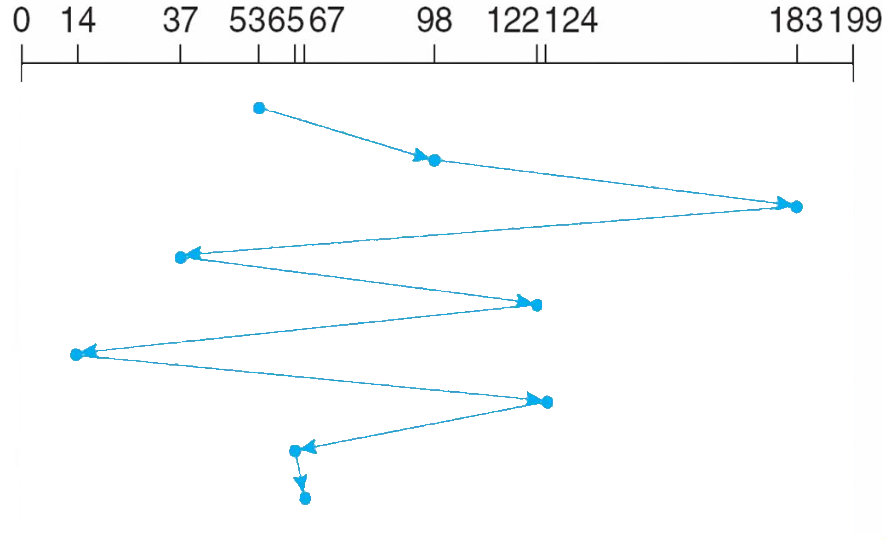
\includegraphics[width=0.5\linewidth]{img/Immagine 2024-05-22 183104.png}
\end{figure}

\subsection{SCAN - elevator algorithm}

The disk arm start at one end of the disk, and moves toward the
other end. This is not equal, the last value have to wait a lot of time.

\begin{figure}[h!]
    \centering
    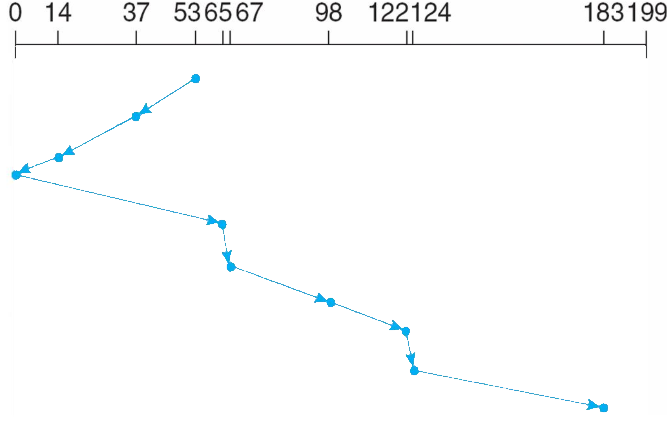
\includegraphics[width=0.5\linewidth]{img/Immagine 2024-05-22 183628.png}
\end{figure}

\paragraph{NOTE: } there are no request from 0-65, we can just skip it.


\subsection{C-SCAN}
Provides a more uniform wait time than SCAN, the head moves from one end of the disk to the other, servicing
requests as it goes. When it reaches the other end, however, it immediately returns to
the beginning of the disk, without servicing any requests on the
return trip.


\begin{figure}[h!]
    \centering
    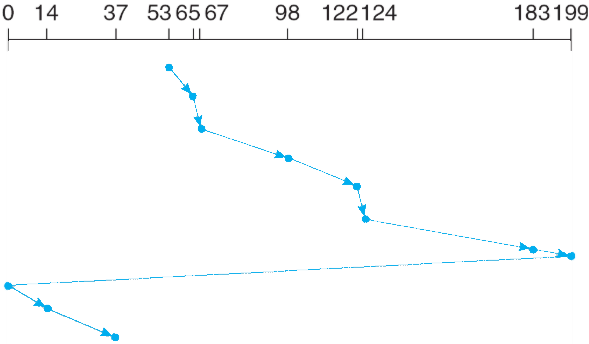
\includegraphics[width=0.5\linewidth]{img/Immagine 2024-05-22 184919.png}
\end{figure}

\newpage
\subsection{Chooseing Disk-Scheduling Algorithm }

\begin{itemize}
    \item FCFS is common and has a natural appeal
    \item SCAN and C-SCAN perform better for systems that place a heavy load on the disk
\end{itemize}

Linux implements deadline scheduler

\begin{itemize}
    \item[-] Maintains separate read and write queues
    \item[-] By default, read batches take precedence over write batches, because applications are more likely to block on read I/O operations.
    \item[-] Schedules read and write batches for execution in increasing logical block addressing (LBA)
    \item[-] After each batch, it naturally select read batches if any, but also checks how long write operations have been waiting (to avoid starvation)
    \item[-] schedules the next read or write batch as appropriate
    \item[-] Typically, if read batch is waiting for more than 500ms, gets priority over read
\end{itemize}

This scheduler is suitable for most use cases, but particularly those in which the
write operations are mostly \textbf{asynchronous}.


\section{NVM Scheduling}
No disk heads or rotational latency but still room for optimization. NVM best at random I/O, HDD at sequential, the Input/Output operations per second (IOPS) much higher with NVM (hundreds of thousands vs hundreds).


\section{Device management}

One fundamental aspect of many parts of computing is the \textbf{Error Detection and Correction}. 

The \textbf{Error detection} determines if there a problem has occurred, frequently used via parity bit. 

Parity one form of checksum and another error-detection method is cyclic
redundancy check (CRC) which uses hash function to detect
multiple-bit errors.

\paragraph{}

\textbf{Error-correction code}, ECC, not only detects, but can correct some
errors, soft errors correctable, hard errors detected but not corrected.


\subsection{Storage Device Management}

\textbf{Low-level formatting}, or \textbf{physical formatting} - dividing a disk into
sectors that the disk controller can read and write. Each sector can hold header information, plus data, plus error
correction code. Usually 512 bytes of data but can be selectable.

To use a disk to hold files, the operating system still needs to record its
own data structures on the disk:

\begin{itemize}
    \item \textbf{Partition} the disk into one or more groups of cylinders, each treated as a logical disk
    \item \textbf{Logical formatting} or “making a file system”
\end{itemize}

To increase efficiency most file systems group blocks into clusters. Disk I/O done in blocks, File I/O done in clusters.


\paragraph{}

\textbf{Boot/root partition} contains the OS, other partitions can hold other Oses, other file systems, or be raw. The partition can be \textbf{mounted} at boot time, or automatically or manually.

At mount time, file system consistency checked, all metadata correct? 

\begin{itemize}
    \item[] If not, fix it, try again
    \item[] If yes, add to mount table, allow access
\end{itemize}

Boot block, or a boot management program for multi-os booting, can point to boot volume or boot loader set of blocks that
contain enough code to know how to load the kernel from the file system.

Boot block initializes system, it is stored in ROM, firmware. The Bootstrap loader program
stored in boot blocks of boot partition, master boot record MBR.

\begin{figure}[h!]
    \centering
    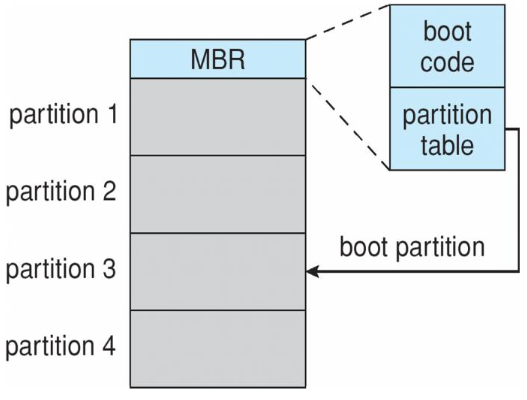
\includegraphics[width=0.37\linewidth]{img/fhmgmfgzh.png}
    \caption{Booting from secondary
storage in Windows}
\end{figure}

\subsection{Swap-Space Management}
Used for moving entire processes or pages from DRAM to secondary
storage when DRAM not large enough for all processes. The Operating system provides \textbf{swap space management}:

\begin{itemize}
    \item Secondary storage slower than DRAM, so important to optimize performance
    \item Usually multiple swap spaces possible – decreasing I/O load on any given device
    \item Best to have dedicated devices
    \item Can be in raw partition or a file within a file system (for convenience of adding)
\end{itemize}


\begin{figure}[h!]
    \centering
    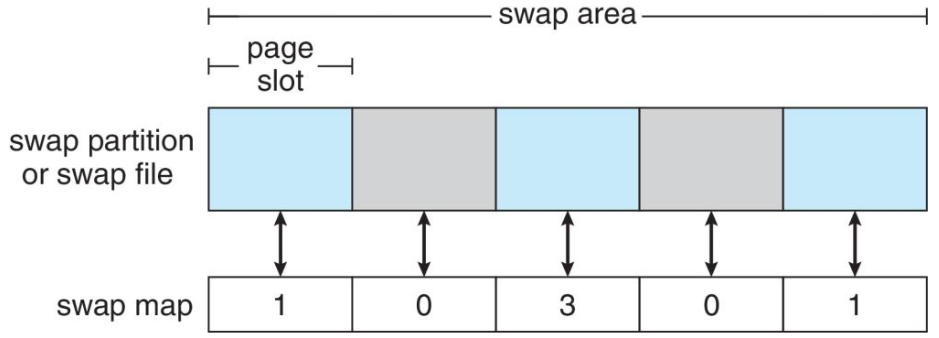
\includegraphics[width=0.55\linewidth]{img/amrjkyt.png}
    \caption{Data structures for swapping on Linux systems}
\end{figure}


\newpage
\subsection{Host Storage Attachment}

Computers access storage in three ways:

\begin{itemize}
    \item[--] host-attached
    \item[--] network-attached
    \item[--] cloud
\end{itemize}

Host attached access through local I/O ports, using one of several
technologies to attach many devices (USB, LAN...).

\subsubsection{Network-Attached Storage: NAS}

Network-attached storage (NAS) is storage made available over a
network rather than over a local channel (such as a bus). \textbf{NFS} and \textbf{CIFS} are common protocols, implemented via remote procedure calls (RPCs) between host and
storage over typically TCP or UDP on IP network.

\begin{figure}[h!]
    \centering
    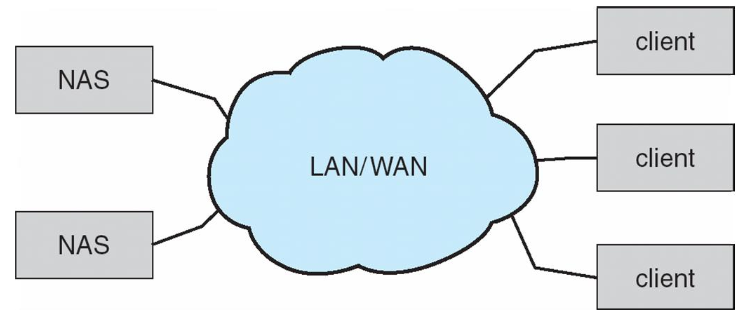
\includegraphics[width=0.5\linewidth]{img/tdmng.png}
    \caption{NAS}
\end{figure}

\subsection{Cloud Storage}

Similar to NAS, provides access to storage across a network. Unlike NAS, accessed over the Internet or a WAN to remote
data center.

NAS presented as just another file system, while cloud storage is
API based, with programs using the APIs to provide access. Use APIs because of latency and failure scenarios (NAS
protocols wouldn’t work well).

\subsection{Redundant Array of Independent Disks - RAID}

RAID - multiple disk drives provides reliability via redundancy. 

\begin{itemize}
    \item Increases the \textbf{mean time to failure}.
    \item \textbf{Mean time to repair} – exposure time when another failure could cause data loss
    \item \textbf{Mean time to data} loss based on above factors
\end{itemize}


If mirrored disks fail independently, consider disk with 100,000 mean
time to failure and 10 hour mean time to repair. The mean time to data loss is:

\begin{equation*}
    \text{MTDL } = 100\,000^2 / (2*10) = 500 * 10^6 \text{ hours or 57 000 years! }   
\end{equation*}

Several improvements in disk-use techniques involve the use of
multiple disks working cooperatively.

\newpage

Disk \textbf{striping} uses a group of disks as one storage unit. RAID is arranged into six different levels.

RAID schemes improve performance and improve the reliability of
the storage system by storing redundant data


\begin{itemize}
    \item \textbf{Mirroring} or shadowing (\textbf{RAID 1}) keeps duplicate of each disk
    \item Striped mirrors (\textbf{RAID 1+0}) or mirrored stripes (\textbf{RAID 0+1}) provides high performance and high reliability
    \item Block interleaved parity (\textbf{RAID 4, 5, 6}) uses much less redundancy
\end{itemize}

RAID within a storage array can still fail if the array fails, so
automatic replication of the data between arrays is common. Frequently, a small number of hot-spare disks are left
unallocated, automatically replacing a failed disk and having data
rebuilt onto them.


\begin{figure}[h!]
    \begin{minipage}[h!]{0.5\textwidth}
        \centering
        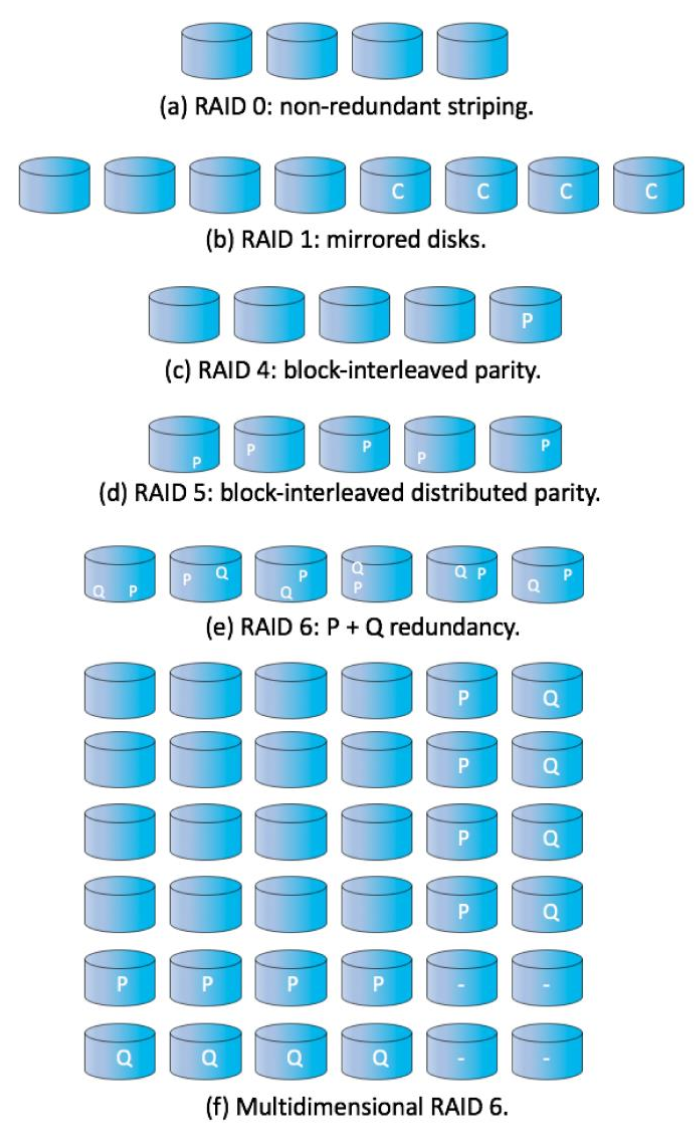
\includegraphics[width=1\linewidth]{img/zmfdg.png}
    \caption{RAID schemes}
    \end{minipage}
    \begin{minipage}[h!]{0.5\textwidth}
    \centering
    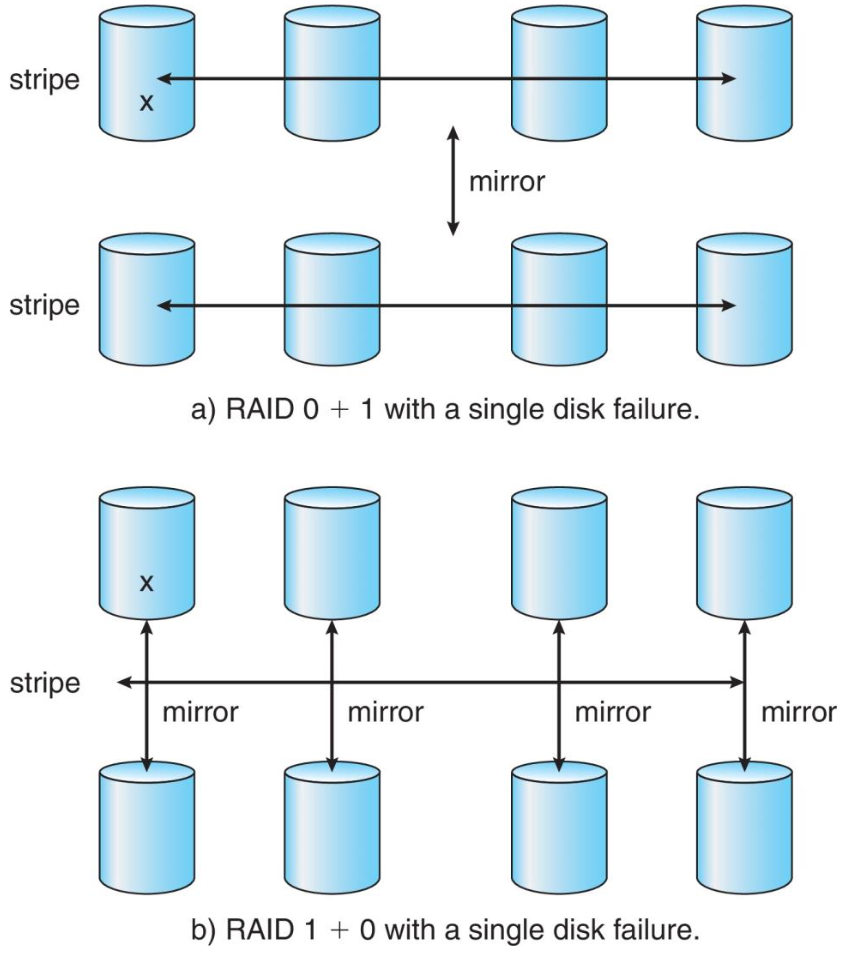
\includegraphics[width=1\linewidth]{img/zmnfdg.png}    
    \end{minipage}
\end{figure}


\chapter{File-System Interface}

\section{What’s a File?}

Contiguous logical address space. Types:

\begin{itemize}
    \item Data File
        \begin{itemize}
        \item Numeric
        \item Character
        \item Binary
        \end{itemize}
    \item Program File
\end{itemize}

\begin{figure}[h!]
    \centering
    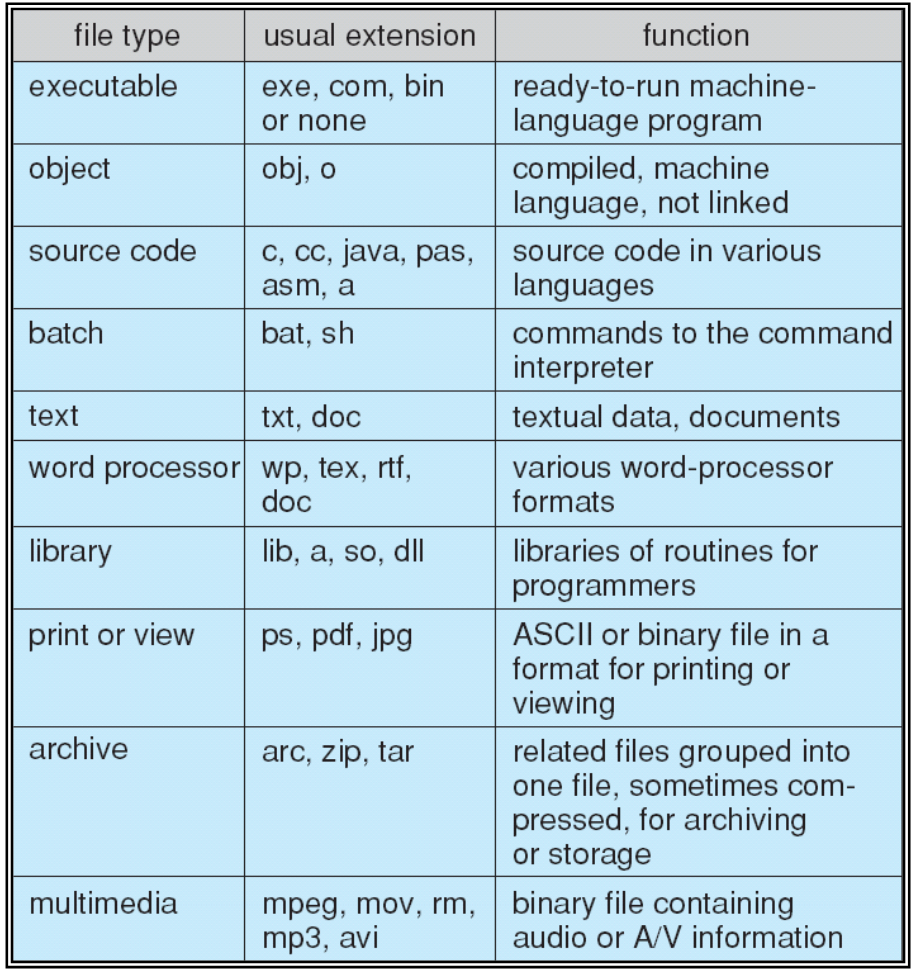
\includegraphics[width=0.5\linewidth]{img/fgnfnfg.png}
    \caption{Type of files}
\end{figure}


\newpage
\subsection{File Attributes}

\begin{itemize}
    \item \textbf{Name} – only information kept in human-readable form
    \item \textbf{Identifier} – unique tag (number) identifies file within file system
    \item \textbf{Type} – needed for systems that support different types
    \item \textbf{Location} – pointer to file location on device
    \item \textbf{Size} – current file size
    \item \textbf{Protection} – controls who can do reading, writing, executing
    \item \textbf{Time}, \textbf{date}, and \textbf{user} \textbf{identification} – data for protection, security, and usage monitoring
\end{itemize}

Information about files are kept in the \textbf{directory structure}, which is
maintained on the disk. Many variations, including extended file attributes such as file checksum.

\subsection{File Structure}

\begin{itemize}
    \item None - sequence of words, bytes
    \item Simple record structure - Lines, Fixed length, Variable length...
    \item Complex Structures - Formatted document Relocatable load file
\end{itemize}

Can simulate last two with first method by inserting appropriate
control characters.

The decision of the structure is up to the \textbf{OS} or \textbf{Program}.

\section{File access and operation}

Several pieces of data are needed to manage \textbf{open files}:

\begin{itemize}
    \item \textbf{Open-file table}: tracks open files
    \item File pointer: pointer to last read/write location, per process that has the file open
    \item \textbf{File-open count}: counter of number of times a file is open – to allow removal of data from open-file table when last processes closes it
    \item Disk location of the file: cache of data access information
    \item Access rights: per-process access mode information
\end{itemize}

\subsection{File Locking}
Provided by some\textbf{ operating systems} and file systems. Similar to reader-writer locks.

\textbf{Shared lock} similar to reader lock – several processes can acquire concurrently
\textbf{Exclusive lock} similar to writer lock

\paragraph{}

\textbf{Mandatory} – access is denied depending on locks held and requested
\textbf{Advisory} – processes can find status of locks and decide what to do

\paragraph{Example: } try to write a file which is already opened in Excel, you get and error; if you try to open a file in gedit, usually not.

\subsection{Access Methods}

A file is fixed length \textbf{logical record(s)}: 

\begin{itemize}
    \item Sequential Access
    \item Direct Access
    \item Other Access Methods
\end{itemize}

\subsubsection{Sequential Access}
Operations: read next, write next, Reset, no read after last write (rewrite), No “seek”.


\begin{figure}[h!]
    \centering
    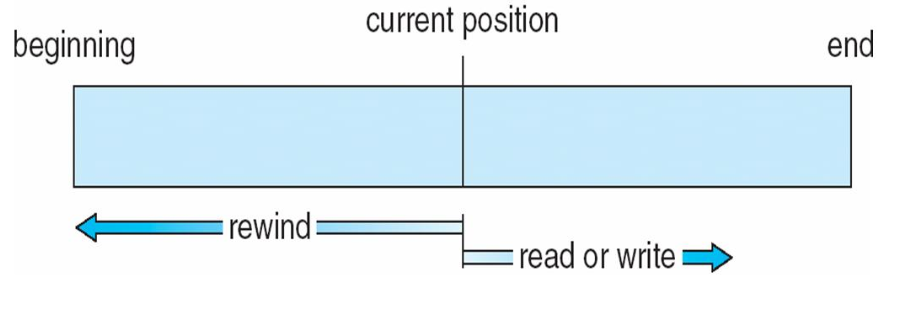
\includegraphics[width=0.45\linewidth]{img/andfg.png}
    \caption{Sequential Access}
\end{figure}

\subsubsection{Direct Access}
Operations: read n, write n, Reset, Position (seek) to n. n = relative block number

\begin{figure}[h!]
    \centering
    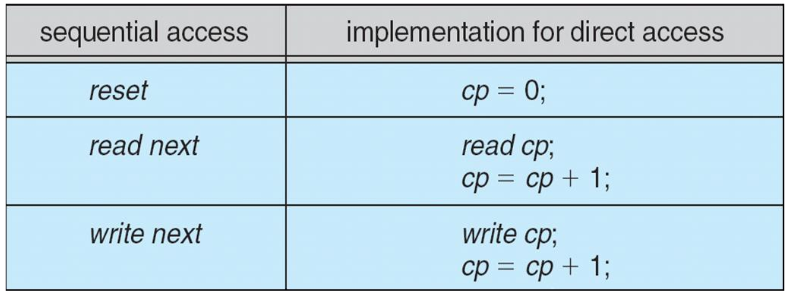
\includegraphics[width=0.5\linewidth]{img/dbfs.png}
    \caption{Direct Access}
\end{figure}

\subsubsection{Sequential vs Direct access}


\begin{figure}[h!]
    \centering
    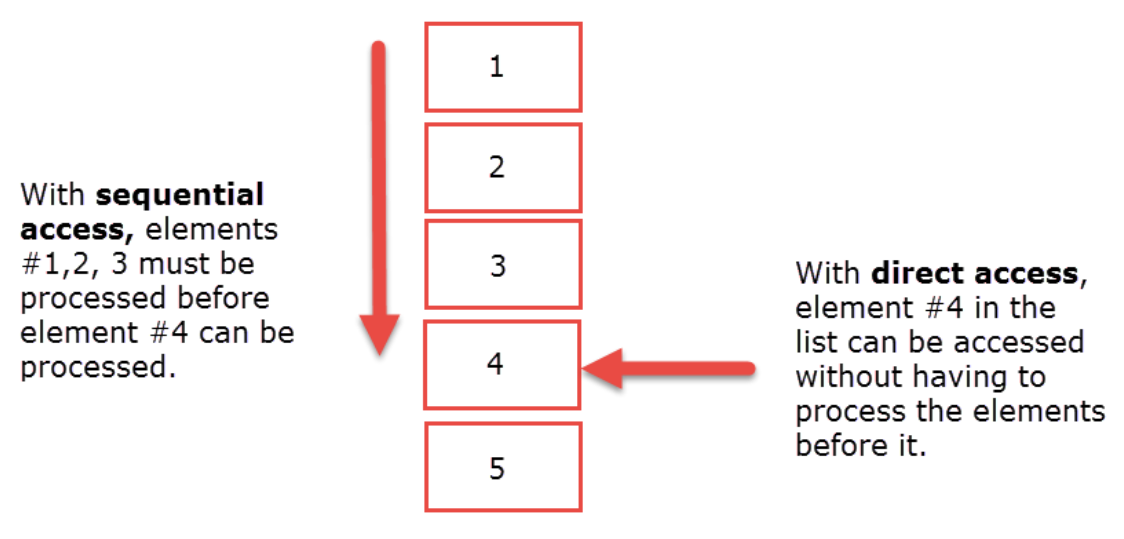
\includegraphics[width=0.5\linewidth]{img/mhfg.png}
\end{figure}

\subsubsection{Other Access Methods}

Can be other access methods built on top of base methods. Generally involve creation of an index for the file. Keep index in memory for fast determination of location of data to be
operated on (consider Universal Produce Code (UPC code) plus record
of data about that item).

If the index is too large, create an in-memory index, which an index of a
disk index.
\paragraph{}
IBM indexed sequential-access method (ISAM)

\begin{itemize}
    \item Small master index, points to disk blocks of secondary index
    \item File kept sorted on a defined key
    \item All done by the OS
    \item A similar engine, MyISAM, is a way of indexing MySQL DBs
\end{itemize}

\begin{figure}[h!]
    \centering
    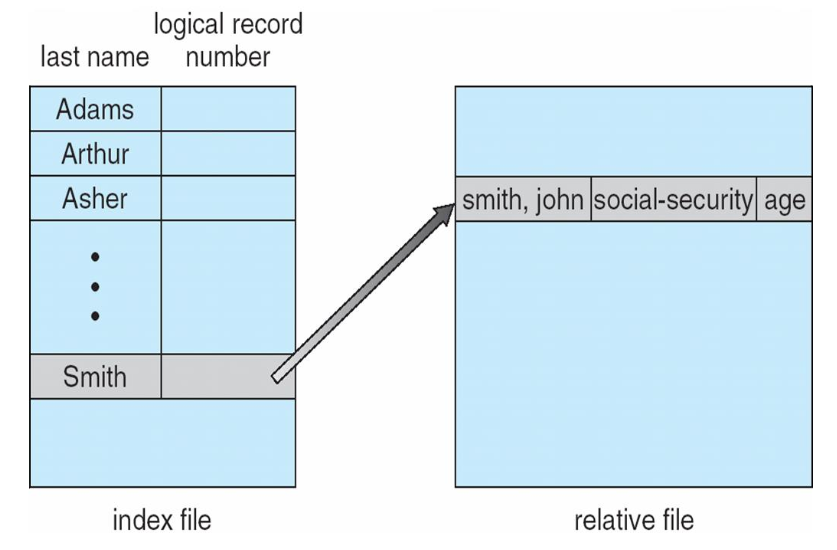
\includegraphics[width=0.5\linewidth]{img/dfb.png}
\end{figure}

\section{Memory-Mapped Files}

Rather than accessing data files from the HD with every file access, data
files can be paged into memory the same as process files, resulting in much
faster accesses.

You can see it as “paging” a file = a page table per file, except of course when page-faults occur. This is known as memory-mapping a file.

\paragraph{}
A file is mapped to an address range within a process's virtual address
space, and then paged in as needed using the ordinary demand paging
system. Can be used to load 10GB file when only 2GB RAM available!

File writes are made to the memory page frames, and are not immediately
written out to disk. This is also why it is important to "close( )" a file when done writing to it.

So that the data can be safely flushed out to disk and so that the
memory frames can be freed up for other purposes.


\begin{figure}[h!]
    \centering
    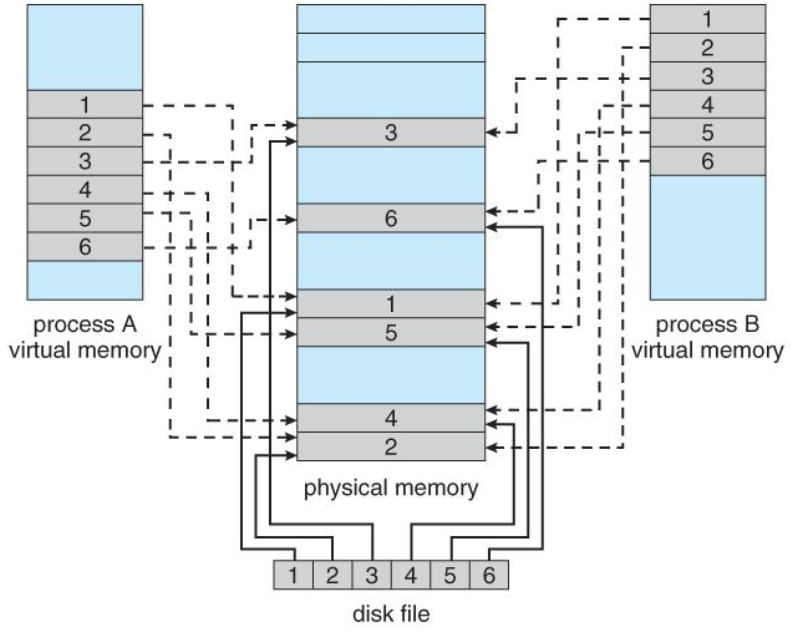
\includegraphics[width=0.5\linewidth]{img/mfh.png}
    \caption{Memory-Mapped Files}
\end{figure}

\newpage
\section{Disk and File Systems}

From last lecture:
\begin{itemize}
    \item Disks can be subdivided into partitions
    \item Disks or partitions can be RAID protected against failure
    \item Partitions also known as minidisks, slices
\end{itemize}

A file system or filesystem (often abbreviated to FS or fs) governs
file organization and access.

Entity containing file system is known as a volume, a formatted disk or partition is a volume.

Disk or partition can be used raw – without a file system, or
formatted with a file system. Each volume containing a file system also tracks that file system’s
info in device directory or volume table of contents. In addition to general-purpose file systems there are many
special-purpose file systems, frequently all within the same
operating system or computer.

\subsection{Types of File Systems}
We mostly talk of general-purpose file systems, but systems frequently have many file systems, some general- and some
special- purpose.

Consider Solaris has:

\begin{itemize}
    \item tmpfs – memory-based volatile FS for fast, temporary I/O
    \item objfs – interface into kernel memory to get kernel symbols for debugging
    \item ctfs – contract file system for managing daemons
    \item lofs – loopback file system allows one FS to be accessed in place of another
    \item procfs – kernel interface to process structures
    \item ufs, zfs – general purpose file systems
\end{itemize}

And also Linux has multiple filesystem.


\section{Directory Structure}
A collection of nodes containing information about all files


\begin{figure}[h!]
    \centering
    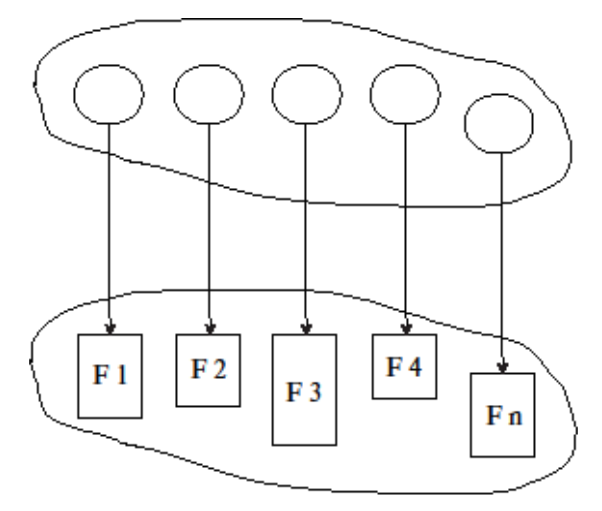
\includegraphics[width=0.4\linewidth]{img/jhg.png}
\end{figure}

 Both the directory structure and the files reside on disk. Directory information are usually on top of a partition.

 \begin{figure}[h!]
     \centering
     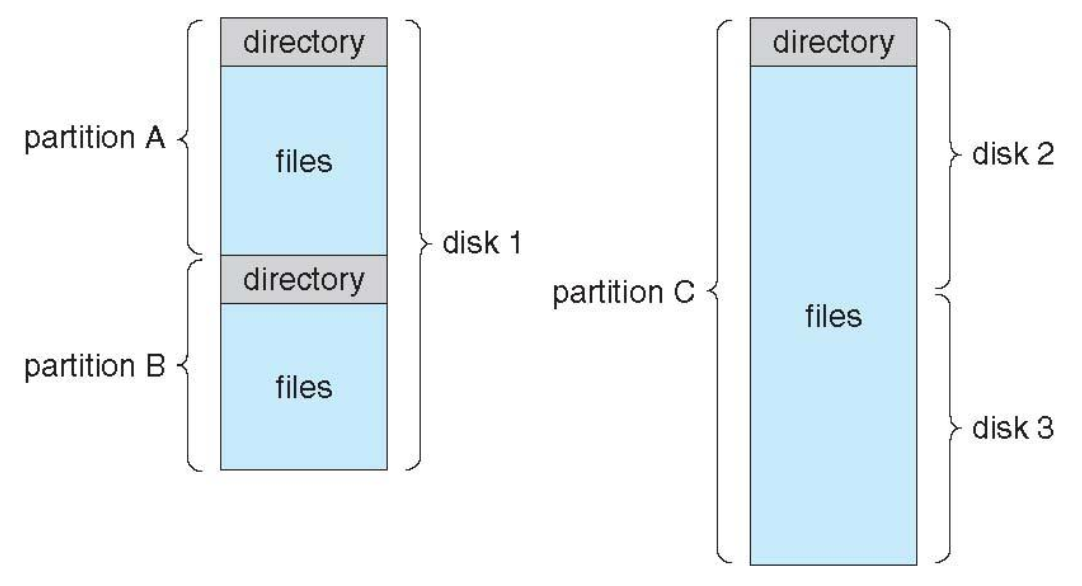
\includegraphics[width=0.5\linewidth]{img/dbgnf.png}
 \end{figure}

 The operation performed on Directory are a lot: Search for a file, Create a file, Delete a file, List contents of a directory, Rename a file, Traverse the file system to sub-directories or parent directories.

 \subsection{Directory Organization}

 The directory is organized logically for performance, usability and access control
Particularly:

\begin{itemize}
    \item Efficiency – locating a file quickly
    \item Naming – convenient to users: Two users can have same name for different files; The same file can have several different names
    \item Grouping – logical grouping of files by properties, (e.g., all Java programs, all games ...)
\end{itemize}

\subsection{Single-Level Directory}

\begin{figure}[h!]
    \centering
    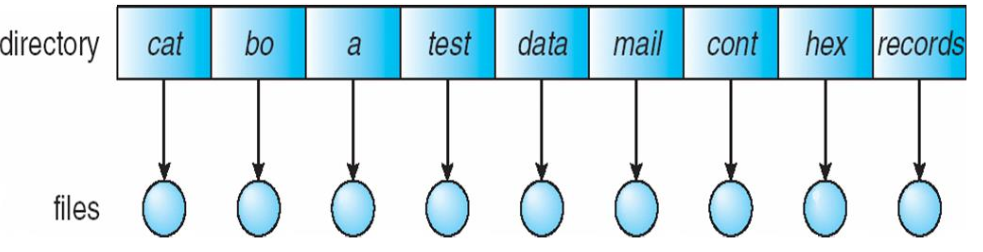
\includegraphics[width=0.5\linewidth]{dfgnb.png}
    \caption{A single directory for all users}
\end{figure}

Lot of problems: Naming problem and Grouping problem are some example.

\subsection{Two-Level Directory}

\begin{figure}[h!]
    \centering
    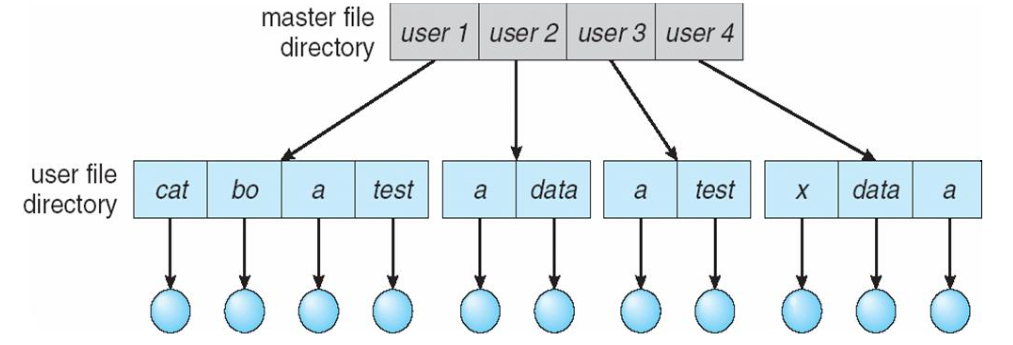
\includegraphics[width=0.5\linewidth]{img/fng.png}
    \caption{Separate directory for each user}
\end{figure}

Features: Long Path name (bad), Can have the same file name for different user (neutral), Efficient searching (good), No grouping capability (bad)

\newpage
\subsection{Tree-Structured Directories}


\begin{figure}[h!]
    \begin{minipage}[h!]{0.5\textwidth}
        \centering
        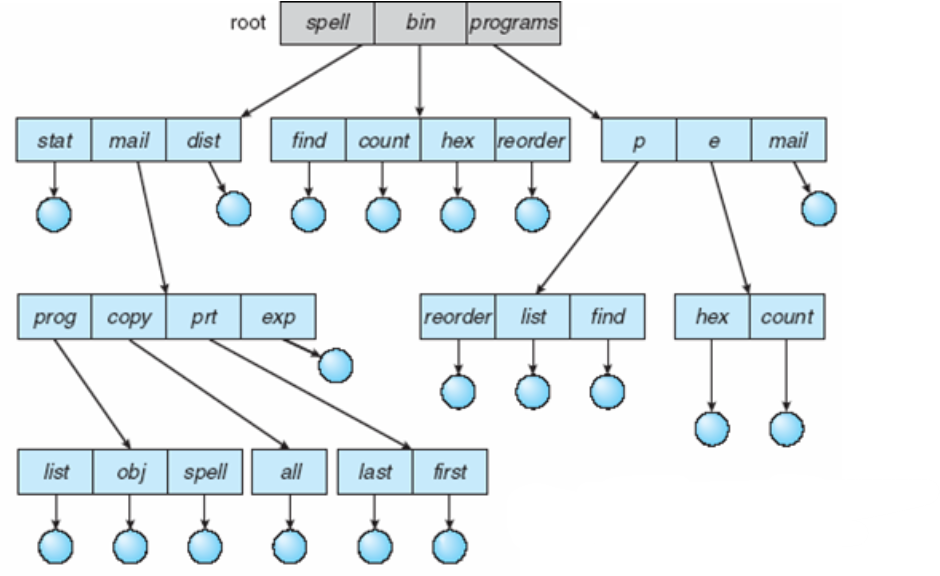
\includegraphics[width=1\linewidth]{img/dfsbv.png}
    \caption{RAID schemes}
    \end{minipage}
    \begin{minipage}[h!]{0.5\textwidth}
    \centering
    \begin{tabular}{c|c}
        Pro & Cons \\
        \hline
        General &Inefficient\\
        Scalable & No file sharing\\
        Easy to Search & File duplication in multiple directories
    \end{tabular}

    \end{minipage}
\end{figure}



\subsection{Acyclic-Graph Directories}

Have shared subdirectories and files with different names (aliases), but may refer to the same data, thus sharing is possible.

\begin{figure}[h!]
    \centering
    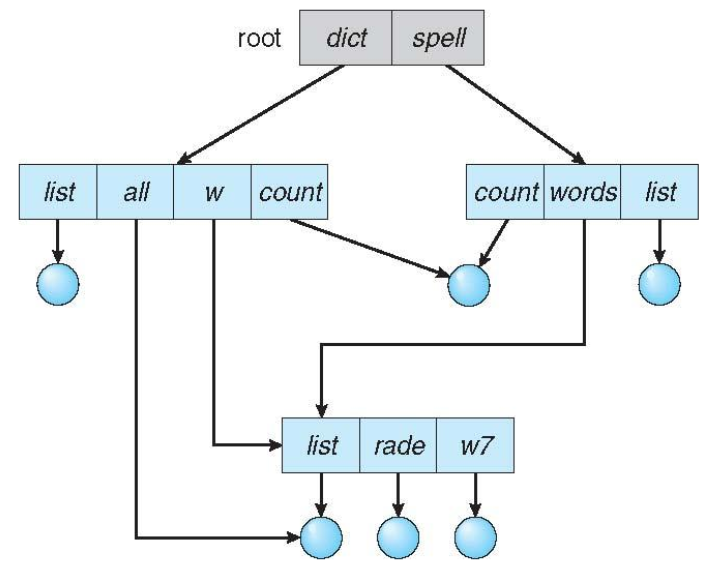
\includegraphics[width=0.5\linewidth]{img/fdbg.png}
\end{figure}

When deleting a directory, you get a dangling pointer that it points to
memory which is no longer allocated, and your dereference of it
constitutes undefined behaviour.

Solutions:

\begin{itemize}
    \item Backpointers, so we can delete all pointers to the deleted folder, variable size records a problem
    \item Backpointers using a daisy chain organization
    \item Entry-hold-count solution
\end{itemize}

New directory entry type:

\begin{itemize}
    \item[] \textbf{Link} – another name (pointer) to an existing file
    \item[] \textbf{Resolve the link} – follow pointer to locate the file
\end{itemize}

\newpage
\subsection{General Graph Directory}

How do we guarantee no cycles? Allow only links to files not sub-directories; \textbf{Garbage collection}; Every time a new link is added use a cycle detection algorithm to
determine whether it is OK.

\begin{figure}[h!]
    \centering
    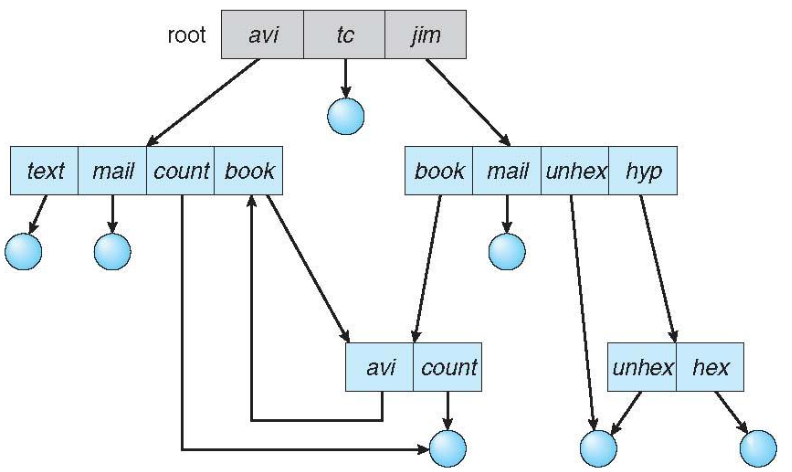
\includegraphics[width=0.55\linewidth]{dngf.png}
\end{figure}

\section{Protection}

The problem:
You don’t want others modifying, reading or moving your
data/programs.

\paragraph{}
 
File owner/creator should be able to control: What can be done/seen, by whom.
Type of access: - Read - Write - Execute - Append - Delete - List.

\paragraph{}
All the OS provide  this basic option.

\chapter{File System Implementation}

\section{File-System Structure}

\textbf{File structure}:  Logical storage unit and collection of related information.

\textbf{File system provides: }

\begin{itemize}
    \item user interface to storage, mapping logical to physical
    \item efficient and convenient access to disk by allowing data to be stored, located retrieved easily
    \item Interface to HW: Disk provides in-place rewrite and random access - I/O transfers performed in blocks or sectors (usually 512 bytes)
\end{itemize}

\textbf{File control block} (\textbf{FCB}) - storage structure consisting of information about a file.

\textbf{Device driver} controls the physical device - Many activities: a File System can be organized into layers.


\section{Layered File System}

\begin{figure}[h!]
    \centering
    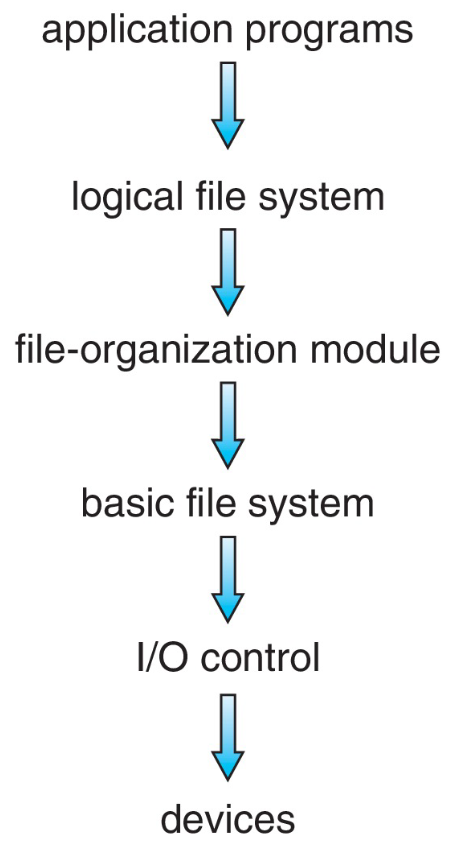
\includegraphics[width=0.25\linewidth]{img/sdfrbn.png}
\end{figure}

\newpage
\subsection{Device drivers}

\textbf{Device drivers} manage I/O devices at the I/O control layer.


Given commands like: read drive1, cylinder 72, track 2, sector 10, into memory location 1060.


Outputs low-level hardware specific commands to hardware controller

\subsection{Basic file system }

\textbf{Basic file system} given command like “retrieve block 123” translates to device
driver.

Also manages memory buffers and caches (allocation, freeing, replacement):
\begin{itemize}
    \item Buffers hold data in transit
    \item Caches hold frequently used data
\end{itemize}





\subsection{File organization module}

\textbf{File organization} \textbf{module} understands files, logical address, and physical
blocks.

Translates logical block \# to physical block \#.

Manages free space, disk allocation.







\subsection{Logical file system}
Logical file system manages metadata information:

\begin{itemize}
    \item Translates file name into file number, file handle, location by maintaining file control blocks (inodes in UNIX)
    \item Directory management
    \item Protection
\end{itemize}

Layering useful for reducing complexity and
redundancy, but adds overhead and can decrease
performance.

Logical layers can be implemented by any coding
method according to OS designer.


The logical file system is directly called by
\textbf{applications} e.g., C open()    






\section{File System Types}

Many file systems, sometimes many within an operating system, each with its own format:
\begin{itemize}
    \item CD-ROM is ISO 9660;
    \item Unix has UFS, FFS;
    \item Linux has more than 130 types, with extended file system ext3 and ext4 leading;
    \item Windows has FAT, FAT32, NTFS as well as floppy, CD, DVD Blu-ray.
\end{itemize}

New ones still arriving – ZFS, GoogleFS, Oracle ASM, FUSE

\newpage

\section{From API to implementation}

\subsection{File-System Operations}

We have system calls at the API level:  Open, close, read, write, seek...but how do we implement their functions? On-disk and in-memory structures.

\paragraph{}
\textbf{Boot control block} (or \textbf{MBR}) contains info needed by system to boot OS from
that volume. Needed if volume contains OS, usually first block of volume.

\textbf{Volume control block} (superblock, master file table) contains volume details: Total \# of blocks, \# of free blocks, block size, free block pointers or array.

Directory structure organizes the files: Names and inode numbers, master file table.

\subsection{File Control Block - FCB}

OS maintains FCB per file, which contains many details about the file: Typically, inode number (if linux), permissions, size, dates.


\begin{figure}[h!]
    \begin{minipage}[h!]{0.5\textwidth}
        \centering
        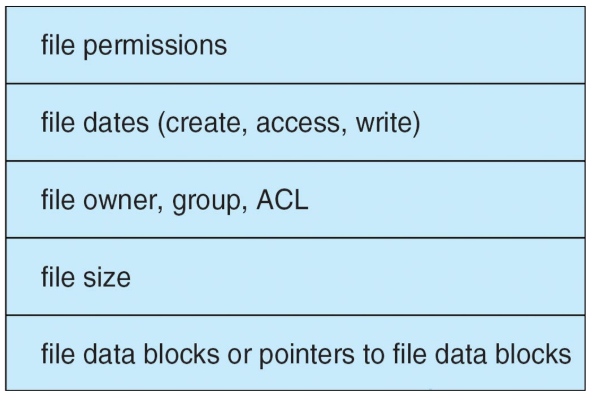
\includegraphics[width=1\linewidth]{img/mfhg.png}
    \end{minipage}
    \begin{minipage}[h!]{0.5\textwidth}
    \centering
    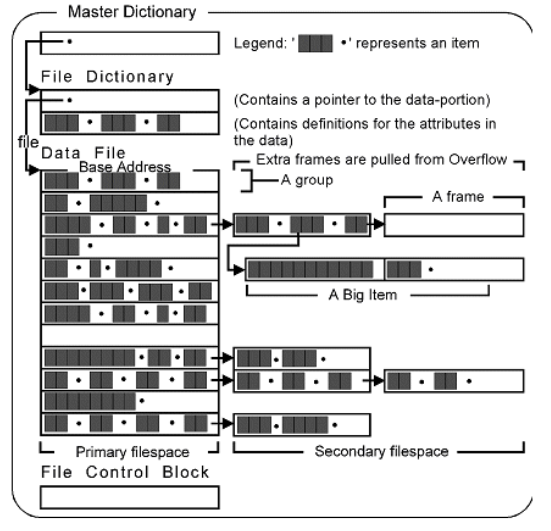
\includegraphics[width=1\linewidth]{img/dfngb.png}     
    \end{minipage}
\end{figure}

\subsection{The Linux iNode}

An inode (aka index node) is a data structure used by Unix/Linux in order to
describe an object within a filesystem. Such an object could be a file or a directory.

Every inode stores pointers to the disk block’s locations of the object’s data and
metadata.

Overall, the metadata contained in an inode is:

\begin{itemize}
    \item file type (regular file/directory/symbolic link/block special file/character special file/etc),
    \item permissions,
    \item owner/group id,
    \item size,
    \item last accessed/modified time,
    \item change time
    \item number of hard links
\end{itemize}


\begin{figure}[h!]
    \begin{minipage}[h!]{0.5\textwidth}
        \centering
        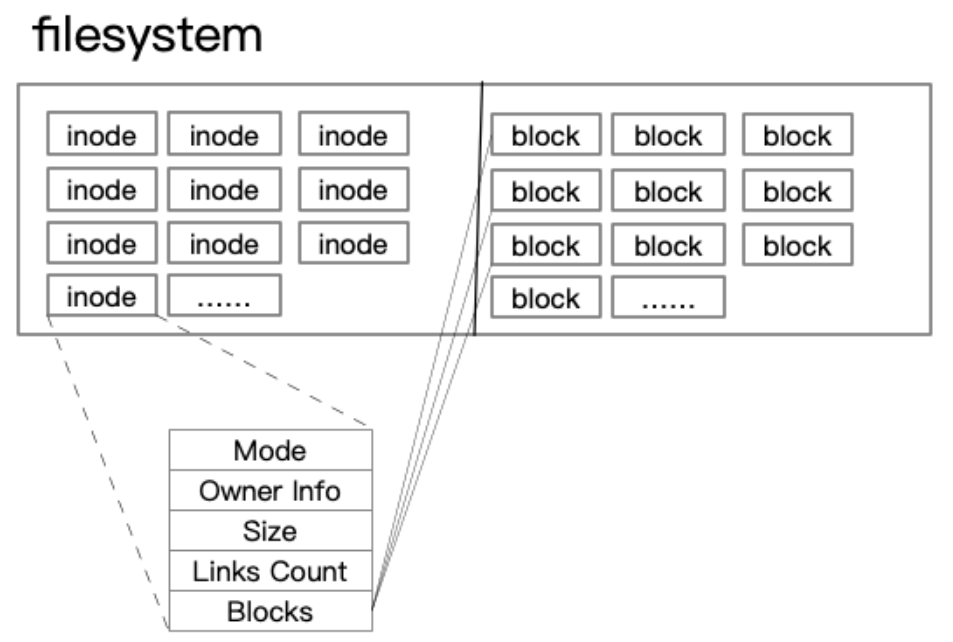
\includegraphics[width=1\linewidth]{img/dfnsb.png}
    \caption{The Linux iNode}
    \end{minipage}
    \begin{minipage}[h!]{0.5\textwidth}
    \centering
    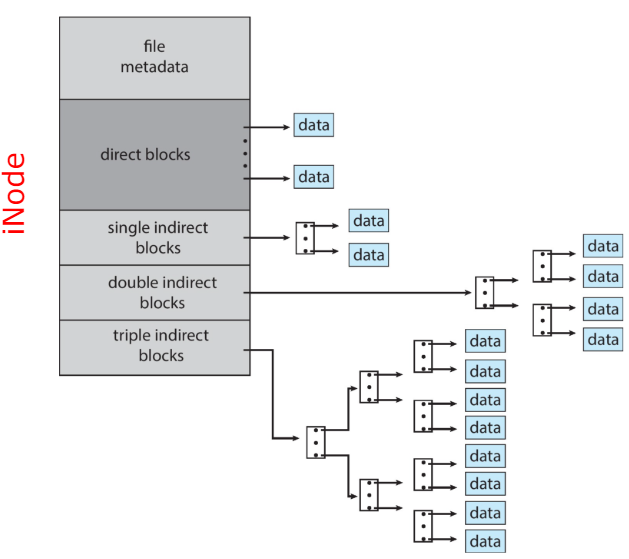
\includegraphics[width=1\linewidth]{img/smgth.png}
    \caption{UNIX UFS - 4K bytes per block, 32-bit addresses} 
    \end{minipage}
\end{figure}


\subsection{In-Memory File System Structures}

\textbf{Mount table} - storing file system mounts, mount points, file system types.

\textbf{System-wide open-file table} - contains a copy of the FCB of each file and other
info.

\textbf{Per-process open-file table} - contains pointers to appropriate entries in systemwide open-file table as well as other info.

\paragraph{}

Items of the table are called:

\begin{itemize}
    \item fd file descriptors in UNIX/Linux
    \item fh file handler in Windows
    \item same naming as C functions
\end{itemize}

\begin{figure}[h!]
    \centering
    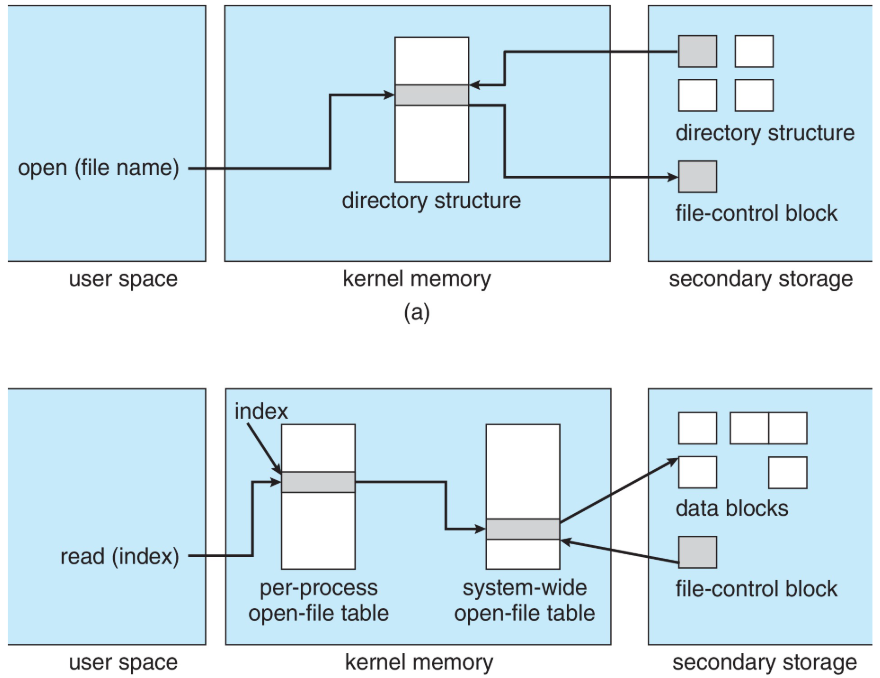
\includegraphics[width=0.5\linewidth]{img/mxfhg.png}
\end{figure}

\newpage
\section{Directory Implementation}

\subsection{Linear}

Linear list of file names with pointer to the data blocks.

\begin{itemize}
    \item Simple to program
    \item Time-consuming to execute,  Linear search time, could keep ordered alphabetically via linked list or use B+ tree
\end{itemize}


\begin{figure}[h!]
    \centering
    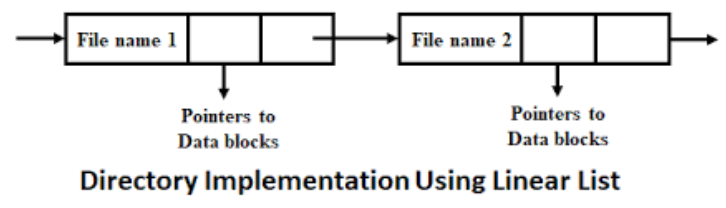
\includegraphics[width=0.5\linewidth]{img/dndsgvg.png}
\end{figure}

\subsection{HashTable}
Hash Table – linear list with hash data structure:
\begin{itemize}
    \item Decreases directory search time
    \item Collisions – situations where two file names hash to the same location
    \item Only good if entries are fixed size, or use chained-overflow method
\end{itemize}


\begin{figure}[h!]
    \centering
    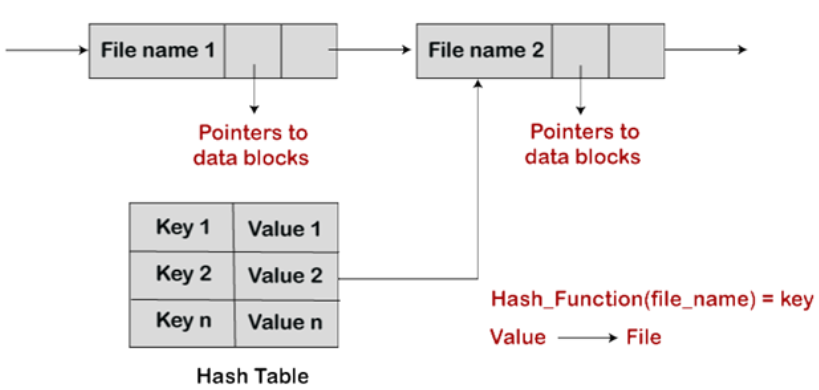
\includegraphics[width=0.5\linewidth]{img/dghgf.png}
\end{figure}

\section{Allocation Method}

An allocation method refers to how disk blocks are allocated for files:

\begin{itemize}
    \item Contiguous
    \item Linked
    \item File Allocation Table (FAT)
\end{itemize}

\newpage
\subsection{Contiguous Allocation Method }

An allocation method refers to how disk blocks are allocated for files: each file occupies set of contiguous blocks.

\begin{itemize}
    \item Best performance in most cases
    \item Simple – only starting location (block \#) and length (number of blocks) are required
    \item Problems include:
    \begin{itemize}
    \item Finding space on the disk for a file,
    \item Knowing file size,
    \item External fragmentation in the HD, need for compaction off-line (downtime) or on-line. This is also called defrag.
    \end{itemize}
\end{itemize}

Mapping from logical to physical (block size = 512 bytes).

\begin{figure}[h!]
    \centering
    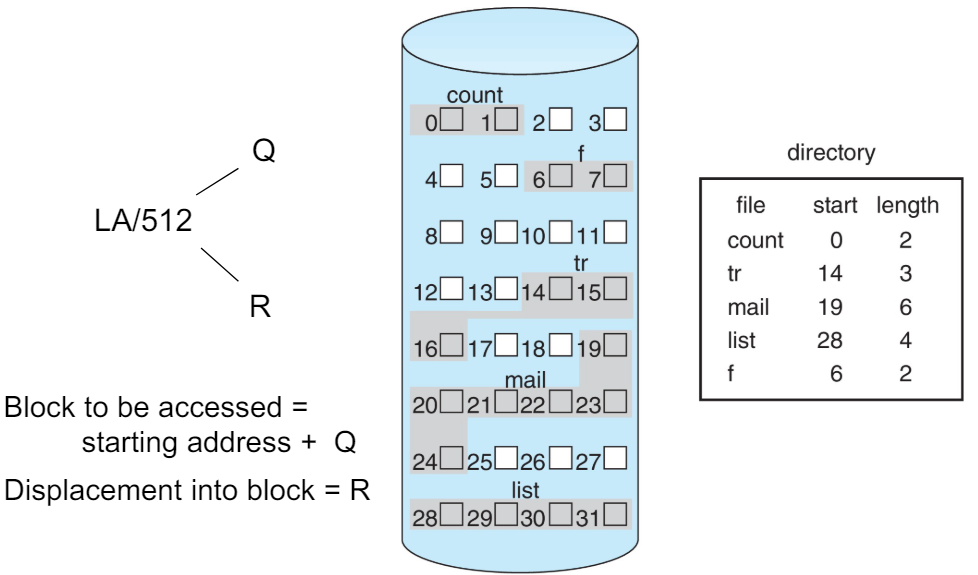
\includegraphics[width=0.6\linewidth]{img/srymkh.png}
\end{figure}


\subsection{Linked Allocation}

\begin{itemize}
    \item[] Each file is a linked list of blocks
    \item[] File ends at nil pointer
    \item[] No external fragmentation
    \item[] Each block contains pointer to next block
    \item[] No compaction, external fragmentation
    \item[] Free space management system called when new block needed
    \item[] Improve efficiency by clustering blocks into groups but increases internal fragmentation
\end{itemize}
\textbf{Big problem}: Locating a block takes many I/Os and disk seeks.

\newpage
Each file is a linked list of disk blocks: blocks may be scattered
anywhere on the disk

\begin{figure}[h!]
    \centering
    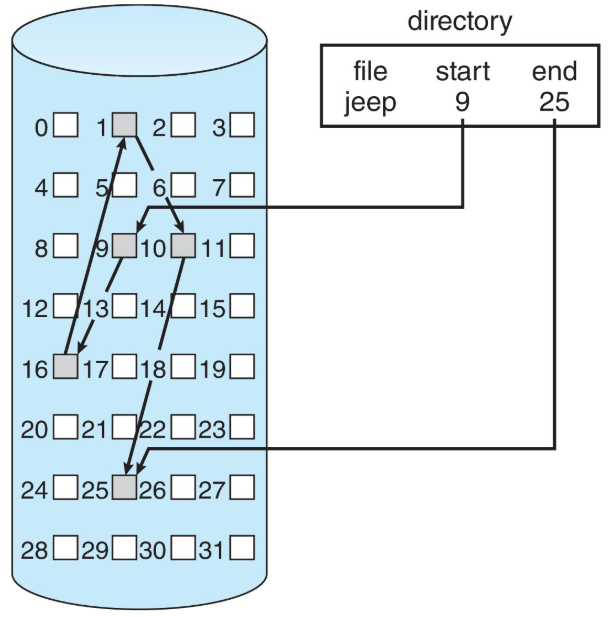
\includegraphics[width=0.4\linewidth]{img/srfymjkgm.png}
\end{figure}

Block to be accessed is the $Q^{th}$ block in the linked chain of
blocks representing the file. Displacement into block = R + 1.

\subsection{FAT Allocation Method}

Beginning of volume has table, indexed by block number. Much like a linked list, but faster on disk and cacheable. New block allocation simple.

\begin{figure}[h!]
    \centering
    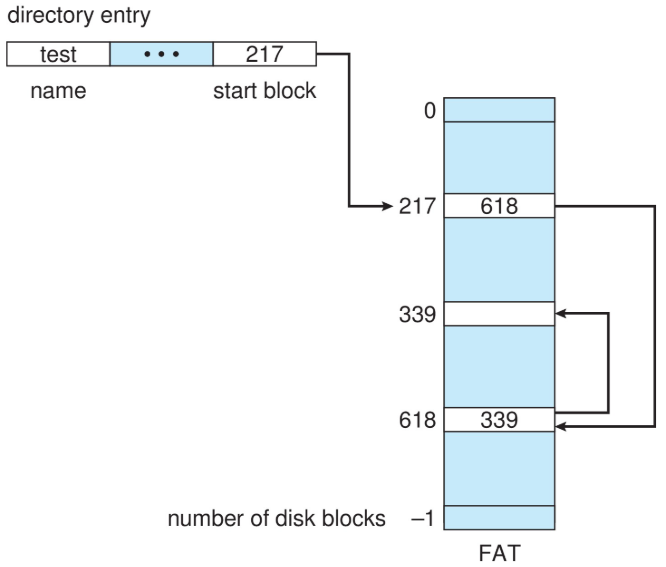
\includegraphics[width=0.5\linewidth]{img/nddgndg.png}
\end{figure}

\newpage
\subsection{Indexed Allocation Method}

Each file has its own index block(s) of pointers to its data blocks.

\begin{figure}[h!]
    \centering
    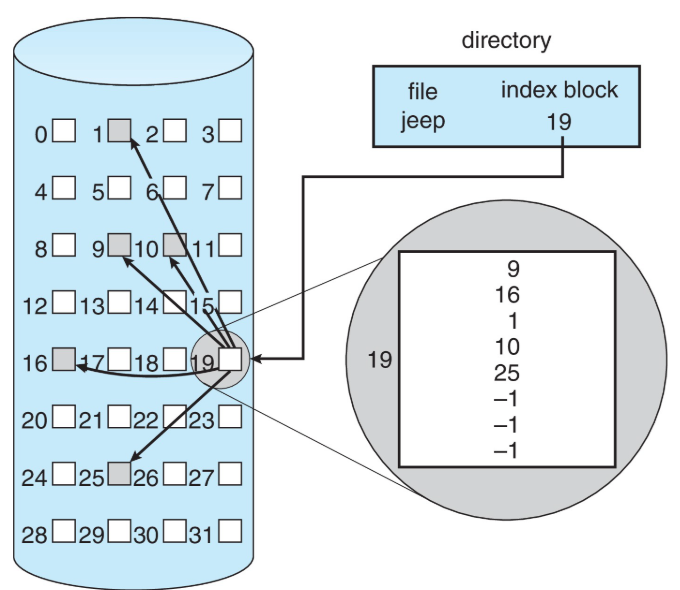
\includegraphics[width=0.5\linewidth]{img/fbfbf.png}
\end{figure}


\subsection{Performance}

Best method depends on file access type:

\begin{itemize}
    \item Contiguous great for sequential and random access
    \item Linked good for sequential, not random
\end{itemize}

Declare access type at creation: select either contiguous or linked.

Indexed more complex: single block access could requires index block read then data block
read.


\section{Free-Space Management}

File system maintains \textbf{free-space list} to track available blocks. Similar to the free pages list for vm management.

\textbf{Bit vector} or \textbf{bit map} (n blocks)

\begin{figure}[h!]
    \centering
    \includegraphics[width=0.45\linewidth]{img/mngaz.png}
\end{figure}

Block number calculation:

\begin{equation*}
    \text{(number of bits per word) * (number of 0-value words) + offset of first 1 bit}
\end{equation*}
Easy, but Bit map requires extra space.

\paragraph{Example: }



\begin{itemize}
\centering
    \item []block size = 4KB = $2^{12}$ bytes
    \item[] disk size = $2^{40}$ bytes (1 TB)
    \item[] n = $2^{40}$/$2^{12}$ = $2^{28}$ bits (or 32MB)
\end{itemize}

Advantage: Easy to get space for contiguous files by checking if enough
adjacent blocks are free

\subsection{Linked Free Space List on Disk}

Linked list (free list):

\begin{itemize}
    \item \textbf{BAD}: Cannot get contiguous space easily
    \item \textbf{GOOD}: No waste. Linked Free Space List on Disk of space
\end{itemize}


\begin{figure}[h!]
    \centering
    \includegraphics[width=0.4\linewidth]{img/andjfgt.png}
\end{figure}



No need to traverse the entire list (if \#
free blocks recorded)

\subsection{Linked Free Space List}

\textbf{Grouping:}

\begin{itemize}
    \item Modify linked list to store address of next n-1 free blocks in first free block, plus a pointer to next block that contains free-blockpointers (like this one)
    \item First n-1 blocks will be free
    \item The n-th will contain pointers to the next n-1 free blocks
\end{itemize}

\textbf{Counting}

\begin{itemize}
    \item Because space is frequently contiguously used and freed, with contiguous-allocation allocation, extents, or clustering. Keep address of first free block and count of following free blocks, free space list then has entries containing addresses and counts
    \item First block of the free list will contain address of next free block + the number of free blocks after this one
    \item Others will be effectively free blocks
\end{itemize}

\section{FS in other OS}

\subsection{Window’s File Systems}

\textbf{NTFS}, also called New Technology File System, is a proprietary journaling file
system developed by Microsoft. 

Starting with Windows NT 3.1, it is the default file system of the Windows
NT family. It superseded File Allocation Table (FAT) as the preferred file
system on Windows and is also supported in Linux and BSD.


\begin{figure}[h!]
    \centering
    \includegraphics[width=0.5\linewidth]{img/dnfga.png}
\end{figure}
\newpage
\textbf{FAT}, also known as File Allocation Table, is a file system developed for
personal computers.


Originally developed in 1977 for use on floppy disks, it was adapted for use on
hard disks and other devices. It is often supported for compatibility reasons by current operating systems
for personal computers and many mobile devices and embedded systems,
allowing the interchange of data between disparate systems.

\paragraph{}
\textbf{FAT32}, a successor of FAT16, was designed by Microsoft as a new file system
version. FAT32 supports an increased number of possible clusters and reuses
most of the existing codes.

\begin{figure}[h!]
    \centering
    \includegraphics[width=0.55\linewidth]{img/zndfg.png}
    \caption{FAT32 File system structure}
\end{figure}


\subsection{The Apple File System}

In 2017, Apple, Inc., released a new file system to replace its 30-year-old HFS+ file system. HFS+ had been stretched to add many new features, but as usual, this process added complexity, along with lines of code, and made adding more features more difficult. Starting from scratch on a blank page allows a design to start with current technologies and methodologies and provide the exact set of features needed.

\paragraph{}

\textbf{Apple File System} (APFS) is a good example of such a design. Its goal is to run on all current Apple devices, from the Apple Watch through the iPhone to the Mac computers. Creating a file system that works in watchOS, I/Os, tvOS, and macOS is certainly a challenge. APFS is feature-rich, including 64-bit pointers, clones for files and directories, snapshots, space sharing, fast directory sizing, atomic safe-save primitives, copy-on-write design, encryp- tion (single- and multi-key), and I/O coalescing. It understands NVM as well as HDD storage.

\paragraph{}

Most of these features we've discussed, but there are a few new concepts worth exploring. \textbf{Space sharing} is a ZFS-like feature in which storage is avail- able as one or more large free spaces (\textbf{containers}) from which file systems can draw allocations (allowing APFS-formatted volumes to grow and shrink). 

\textbf{Fast directory sizing} provides quick used-space calculation and updating. \textbf{Atomic safe-save} is a primitive (available via API, not via file-system com- mands) that performs renames of files, bundles of files, and directories as single atomic operations. I/O coalescing is an optimization for NVM devices in which several small writes are gathered together into a large write to optimize write performance.
\paragraph{}
Apple chose not to implement RAID as part of the new APFS, instead depending on the existing Apple RAID volume mechanism for software RAID. APFS is also compatible with HFS+, allowing easy conversion for existing deployments.

\chapter{Other File
Systems}

\section{File Sharing}

\textbf{Allows multiple users} / systems access to the same files.

\textbf{Permissions} / protection must be implemented and accurate

\begin{itemize}
    \item Most systems provide concepts of owner, group member
    \item Must have a way to apply these between systems
\end{itemize}

Owner can change attributes and grant access to other users/groups


Group defines a subset of users who can share access to the file.

\paragraph{}

\href{https://www.geeksforgeeks.org/how-to-create-a-shared-folder-between-two-local-user-in-linux/}{Example for creating a shared folder between users} 


\section{Remote File Systems}

Sharing files across a network. First method involved manually sharing each file – programs like \textbf{ftp}.

\begin{figure}[h!]
    \centering
    \includegraphics[width=0.45\linewidth]{img/dfnnfdf.png}
\end{figure}



Second method uses a \textbf{distributed file system} (\textbf{DFS}). Remote directories visible from local machine.

\begin{figure}[h!]
    \centering
    \includegraphics[width=0.65\linewidth]{img/fsdbfbsfbs.png}
\end{figure}

\section{Client-Server Model}

Sharing between:
\begin{itemize}
    \item[--] a server (providing access to a file system via a network protocol) and
    \item[--] a client (using the protocol to access the remote file system)
\end{itemize}

NFS an example:

\begin{itemize}
    \item[--] User auth info on clients and servers must match (UserIDs for example)
    \item[--] Remote file system mounted, file operations sent on behalf of user across network to server
    \item[--] Server checks permissions, file handle returned
    \item[--] Handle used for reads and writes until file closed
\end{itemize}

\begin{figure}[h!]
    \centering
    \includegraphics[width=0.6\linewidth]{img/fdsbdfgbn.png}
\end{figure}

\section{Distributed Information Systems - DIS}

Aka \textbf{distributed naming services}, provide unified access to info needed for
remote computing.

\textbf{Domain name system} (\textbf{DNS}) provides host-name-to-network-address
translations for the Internet

\begin{figure}[h!]
    \centering
    \includegraphics[width=0.46\linewidth]{img/adzgtndrftgn.png}
\end{figure}

Others like network information service (NIS) provide user-name, password,
userID, group information.
\paragraph{}

Microsoft’s common Internet file system (CIFS) network info used with user
auth to create network logins that server uses to allow to deny access:

\begin{itemize}
    \item Active directory distributed naming service
    \item Kerberos-derived network authentication protocol
\end{itemize}

Industry moving toward lightweight directory-access protocol (LDAP) as
secure distributed naming mechanism

\begin{figure}[h!]
    \centering
    \includegraphics[width=0.6\linewidth]{img/sdfbfbs.png}
\end{figure}



\section{Consistency Semantics}

Important criteria for evaluating file sharing-file systems. Specify how multiple users are to access shared file simultaneously.

\textbf{Remember reader-writer?}
\begin{itemize}
    \item [] When modifications of data will be observed by other users
    \item [] Directly related to process synchronization algorithms, but atomicity across a network has high overhead (see Andrew File System)
\end{itemize}

The series of accesses between file open and closed called \textbf{file session}.

UNIX semantics:
\begin{itemize}
    \item Writes to open file immediately visible to others with file open
    \item One mode of sharing allows users to share pointer to current I/O location in file
    \item Single physical image, accessed exclusively, contention causes process delays
\end{itemize}


\section{Virtual File Systems}

\textbf{Virtual File Systems} (\textbf{VFS}) on Unix provide an object-oriented way of
implementing file systems.

VFS allows the same system call interface (the API) to be used for
different types of file systems:


\begin{itemize}
    \item Separates file-system generic operations from implementation details
    \item Implementation can be one of many file systems types, or network file system, implements vnodes which hold inodes or network file details
    \item Then dispatches operation to appropriate file system implementation routines
\end{itemize}

The API is to the VFS interface, rather than any specific type of file
system


\begin{figure}[h!]
    \centering
    \includegraphics[width=0.55\linewidth]{img/dfnhbfd.png}
\end{figure}
\newpage
\subsection{Virtual File System Implementation}

For example, Linux has four object types:

\begin{align*}
    inode, file, superblock, dentry
\end{align*}
VFS defines set of operations on the objects that must be implemented. Every object has a pointer to a function table:

Function table has addresses of routines to implement that function on that object.

For example:
\begin{itemize}
    \item int open(. . .)— Open a file
    \item int close(. . .)— Close an already-open file
    \item ssize t read(. . .)— Read from a file
    \item ssize t write(. . .)— Write to a file
    \item int mmap(. . .)— Memory-map a file
\end{itemize}

\chapter{Virtualization and Virtual Machines}

\section{Virtualization}
Remember what we just said about virtual FSs?

\begin{itemize}
    \item an abstract layer on top of one or more “real” more concrete FSs.
    \item allows client applications to access different types of concrete file systems in a uniform way.
    \item Example: access local and network storage devices transparently without the client application noticing the difference.
    \item It can be used to bridge the differences in Windows, classic Mac OS/macOS and Unix filesystems, so that applications can access files on local file systems of those types without having to know what type of file system they are accessing.
\end{itemize}


\textbf{This is one example of a more general process that is called virtualization.}

\paragraph{}

More in general, Virtualization aims at putting a layer between the
implementation of “something” and its interface / client application /
service.

For FSs, the user does not care about where a file is or how a filesystem is structured, it just uses the APIs. 

This is so nice that it has been extended for “virtualizing” many other
things: and particularly relevant for this course, we can virtualize OSs or Hardware or other devices

\section{Virtual machines}
Fundamental idea – abstract hardware of a single computer into
several different execution environments.

Similar to layered approach, but layer creates virtual system (virtual machine, or VM) on
which operation systems or applications can run.

\paragraph{}

Several components:

\begin{itemize}
    \item \textbf{Host} – underlying hardware system
    \item \textbf{Virtual machine manager} (\textbf{VMM}) or \textbf{hypervisor} – creates and runs virtual machines by providing correct interfacing
    \item \textbf{Guest} – process provided with virtual copy of the host. Usually an operating system
\end{itemize}

Single physical machine can run multiple operating systems concurrently, each in its own virtual machine.

\begin{figure}[h!]
    \centering
    \includegraphics[width=0.55\linewidth]{img/ndfzgdgzfng.png}
    \caption{ (a) Nonvirtual machine. (b) Virtual machine.}
\end{figure}

\subsection{Implementation of VMMs}
Vary greatly, with options including:

\begin{itemize}
    \item \textbf{Type 0 hypervisors} - Hardware-based solutions that provide support for virtual machine creation and management via firmware. They come with the SoC or motherboard. (IBM LPARs and Oracle LDOMs are examples)
    \item \textbf{Type 1 hypervisors} - Operating-system-like software built to provide virtualization. (ex. VMware ESX, Joyent SmartOS, and Citrix XenServer).
    \begin{itemize}
    \item Also includes general-purpose operating systems that provide standard functions as well as VMM functions. Including Microsoft Windows Server with HyperV and RedHat Linux with KVM
    \end{itemize}
    \item \textbf{Type 2 hypervisors} - Applications that run on standard operating systems but provide VMM features to guest operating systems. (VMware / Oracle Virtualbox)
\end{itemize}

\begin{figure}[h!]
    \centering
    \includegraphics[width=0.6\linewidth]{img/dfsnbndbfg.png}
\end{figure}


\subsection{Implementation of VMMs}

Other variations include: 

\begin{itemize}
    \item Paravirtualization - Technique in which the guest operating system is modified to work in cooperation with the VMM to optimize performance
    \item Emulators – Allow applications written for one hardware environment to run on a very different hardware environment, such as a different type of CPU. E.g., IDEs for assembly coding
    \item Application containment - Not virtualization at all but rather provides virtualization-like features by segregating applications from the operating system, making them more secure, manageable. Baseline for sandboxing
\end{itemize}

\subsection{Benefits and Features}

\textbf{Host system protected} from VMs, VMs protected from each other:
\begin{itemize}
    \item A virus less likely to spread
    \item Sharing is provided though via shared file system volume, network communication
\end{itemize}


Freeze, \textbf{suspend}, running VM:

\begin{itemize}
    \item Then can move or copy somewhere else and resume
    \item Snapshot of a given state, able to restore back to that state, some VMMs allow multiple snapshots per VM
    \item Clone by creating copy and running both original and copy
\end{itemize}

\noindent Great for OS \textbf{research}, better system development efficiency.

\vspace{1em}

\noindent Run \textbf{multiple}, different \textbf{OSes} on a single machine, \textbf{consolidation}, app dev.

\vspace{1em}
\noindent \textbf{Templating} – create an OS + application VM, provide it to customers, use it to create multiple instances of that combination.

\vspace{1em}
\noindent \textbf{Live migration} – move a running VM from one host to another! No interruption of user access.

\subsection{Running mode}
Dual mode CPU means guest executes in user mode:

\begin{itemize}
    \item[] Kernel runs in kernel mode
    \item[] Not safe to let guest kernel run in kernel mode too
    \item[] So VM needs two modes – virtual user mode and virtual kernel mode. Both of which run in real user mode
    \item[] Actions in guest that usually cause switch to kernel mode must cause switch to virtual kernel mode
\end{itemize}

\subsection{Trap-and-Emulate}
How does switch from virtual user mode to virtual kernel mode occur?

\begin{itemize}
    \item Attempting a privileged instruction in user mode causes an error $\to$ trap
    \item VMM gains control, analyzes error, executes operation as attempted by guest
    \item Returns control to guest in user mode
    \item Known as trap-and-emulate
    \item Most virtualization products use this at least in part
\end{itemize}

User mode code in guest runs at same speed as if not a guest.

\begin{figure}[h!]
    \centering
    \includegraphics[width=0.45\linewidth]{fdnbfdnb.png}
    \caption{Trap-and-Emulate Virtualization Implementation}
\end{figure}
\newpage
\subsection{What about Containers?}

The last decade has seen a wide spreading of containers:

\begin{itemize}
    \item Which are a way of putting software into “boxes”
    \item makes it very easy to package and ship programs
    \item And bring your code here and there without worrying too much
\end{itemize}

So\dots Containers = Virtual Machines?

\begin{itemize}
    \item[] Short answer: no, but it is a way to virtualize
    \item[] Main difference: containers use a shared OS.
    \item[] Instead of virtualizing hardware as virtual machines, containers rest on top of a single Linux instance.
\end{itemize}

\begin{figure}[h!]
    \centering
    \includegraphics[width=0.6\linewidth]{img/dfvbsvbdfs.png}
    \caption{Containers vs. VMs}
\end{figure}

\newpage
\section{Types of VMS and implementations}
Many variations as well as HW details. Assume VMMs take advantage of HW features, HW features can simplify implementation, improve
performance.

Whatever the type, a VM has a lifecycle:
\begin{enumerate}
    \item Created by VMM
    \item Resources assigned to it (number of cores, amount of memory, networking details, storage details). In type 0 hypervisor, resources usually dedicated, other types dedicate or share resources, or a mix.
    \item When no longer needed, VM can be deleted, freeing resources
\end{enumerate}

Steps simpler, faster than with a physical machine install. Can lead to \textbf{virtual machine sprawl} with lots of VMs, history and state difficult to track.

\subsection{Type 0 Hypervisor}

Old idea, under many names by HW manufacturers: "partitions", "domains", A HW feature implemented by firmware, OS need nothing special, VMM is in firmware, Smaller feature set than other types, Each guest has dedicated HW.

I/O a challenge as difficult to have enough devices, controllers to dedicate to each guest.

Sometimes VMM implements a control partition running daemons
that other guests communicate with for shared I/O.

Can provide virtualization-within-virtualization (guest itself can be a
VMM with guests. Other types have difficulty doing this.


\begin{figure}[h!]
    \centering
    \includegraphics[width=0.5\linewidth]{img/dvsvdsadv.png}
\end{figure}

\subsection{Type 1 Hypervisor}
Commonly found in company datacenters. In a sense becoming “datacenter operating systems”:

\begin{itemize}
    \item Datacenter managers control and manage OSes in new, sophisticated ways by controlling the Type 1 hypervisor
    \item Move guests between systems to balance performance
    \item Snapshots and cloning
\end{itemize}

Another variation is a general purpose OS that also provides VMM functionality:

\begin{itemize}
    \item [] RedHat Enterprise Linux with KVM, Windows with Hyper-V, Oracle Solaris
    \item [] Perform normal duties as well as VMM duties
    \item [] Typically less feature rich than dedicated Type 1 hypervisors
\end{itemize}



In many ways, treat guests OSes as just another process. Albeit with special handling when guest tries to execute special
instructions.


\subsection{Type 2 Hypervisor}

Less interesting from an OS perspective.

\begin{itemize}
    \item Very little OS involvement in virtualization
    \item VMM is simply another process, run and managed by host, even the host doesn’t know they are a VMM running guests
    \item Tend to have poorer overall performance because can’t take advantage of some HW features
    \item But also a benefit because require no changes to host OS
\end{itemize}

Student could have Type 2 hypervisor on native host, run
multiple guests, all on standard host OS such as Windows,
Linux, MacOS.

\textbf{That’s what we are using for exercises}


\begin{figure}[h!]
    \centering
    \includegraphics[width=0.55\linewidth]{img/dfsvbdfsvb.png}
    \caption{VMware Workstation Architecture}
\end{figure}


\subsection{Programming Environment Virtualization}
Programming language is designed to run within custom-built
virtualized environment. For example Oracle Java has many features that depend on
running in \textbf{Java Virtual Machine} (JVM).
\paragraph{}

In this case virtualization is defined as providing APIs that define a set
of features made available to a language and programs written in that
language to provide an improved execution environment.

\begin{itemize}
    \item JVM compiled to run on many systems (including some smart phones even)
    \item Programs written in Java run in the JVM no matter the underlying system
    \item Similar to interpreted languages
\end{itemize}

\begin{figure}[h!]
    \centering
    \includegraphics[width=0.5\linewidth]{img/fsbbfdvsbfs.png}
    \caption{The Java Virtual Machine}
\end{figure}

Oracle containers / zones for example create virtual layer between OS and apps. Only one kernel running – host OS. OS and devices are virtualized, providing resources within zone
with impression that they are only processes on system. Each zone has its own applications; networking stack, addresses,
and ports; user accounts, etc. CPU and memory resources divided between zones. Zone can have its own scheduler to use those resources.


\section{Virtualization Issues}

Now look at operating system aspects of virtualization. CPU scheduling, memory management, I/O, storage, and unique
VM migration feature.

\begin{itemize}
    \item[] How do VMMs schedule CPU use when guests believe they have dedicated CPUs?
    \item[] How can memory management work when many guests require large amounts of memory?
\end{itemize}

\section{CPU scheduling}

Even single-CPU systems act like multiprocessor ones when
virtualized, one or more virtual CPUs per guest.

Generally VMM has one or more physical CPUs and number of
threads to run on them. Guests configured with certain number of VCPUs.

When enough CPUs for all guests -> VMM can allocate dedicated
CPUs, each guest much like native operating system managing its
CPUs. Usually not enough CPUs -> CPU overcommitment.

VMM can use standard scheduling algorithms to put threads on
CPUs.

\paragraph{}
Cycle stealing by VMM and oversubscription of CPUs means guests
don’t get CPU cycles they expect. Some VMMs provide application to run in each guest to fix time-ofday and provide other integration features

If you cant have dedicated CPU(s) for your guest OS, don’t run a realtime guest OS!

\section{I/O}
Easier for VMMs to integrate with guests because I/O has lots of
variation. Already somewhat segregated / flexible via device drivers, VMM can provide new devices and device drivers.


But overall I/O is complicated for VMMs:

\begin{itemize}
    \item Many short paths for I/O in standard OSes for improved performance
    \item Less hypervisor needs to do for I/O for guests, the better
    \item Possibilities include direct device access, DMA pass-through, direct interrupt delivery. Again, HW support needed for these
\end{itemize}

Networking also complex as VMM and guests all need network access. VMM can bridge guest to network (allowing direct access), and / or provide network address translation (NAT)\footnote{NAT address local to machine on which guest is running, VMM
provides address translation to guest to hide its address}


\section{Storage Management}

Both boot disk and general data access need be provided by VMM. Need to support potentially dozens of guests per VMM (so standard
disk partitioning not sufficient).


\textbf{Type 1} – storage guest root disks and config information within file
system provided by VMM as a disk image.
\textbf{Type 2 }– store as files in file system provided by host OS.
Duplicate file $\to$ create new guest.
Move file to another system $\to$ move guest.

\paragraph{}
\textbf{Physical-to-virtual} (P-to-V) convert native disk blocks into VMM format.

\textbf{Virtual-to-physical} (V-to-P) convert from virtual format to native or disk format.

VMM also needs to provide access to network attached storage (just
networking) and other disk images, disk partitions, disks, etc.


\chapter{Security \& Protection}

\section{What's security? The security problem}

System secure if resources used and accessed as intended under all
circumstances: \textbf{Unachievable}.

\begin{itemize}
    \item \textbf{Intruders} (\textbf{crackers}) attempt to breach security
    \item \textbf{Threat} is potential security violation
    \item \textbf{Attack} is attempt to breach security, attack can be accidental or malicious.
\end{itemize}

Easier to protect against accidental than malicious misuse

\section{Security Violation Categories}

\begin{itemize}
    \item Breach of \textbf{confidentiality}
    \begin{itemize}
        \item[] Unauthorized access to data
    \end{itemize}
    \item Breach of \textbf{integrity}
        \item[] \begin{itemize}
    \item Unauthorized modification/destruction of data
    \end{itemize}
    \item Breach of \textbf{availability}
    \begin{itemize}
        \item[] System/service is not ready for users
    \end{itemize}
\end{itemize}

\section{Example of attacks}

\begin{itemize}
    \item \textbf{Ransomware} (breach integrity) - Encrypts data unless money gets paid to the attacker
    \item \textbf{Replay attack} - Re-send a message as is or with message modification
    \item \textbf{Man-in-the-middle} attack - Intruder sits in data flow, masquerading as sender to receiver and vice versa
    \item \textbf{Session hijacking} - Intercept an already-established session to bypass authentication
    \item \textbf{Privilege escalation} - Common attack type with access beyond what a user or resource is supposed to have
    \item \textbf{Trojan Horse} - Exploits mechanisms for allowing programs written by users to be executed by other users, Spyware, pop-up browser windows
    \item \textbf{Trap Door} - Specific user identifier or password that circumvents normal security procedures, could be included in a compiler Malware - Software designed to exploit, disable, or damage computer
    \item \textbf{Spyware} – Program frequently installed with legitimate software to display adds, capture user data
\end{itemize}

\section{Security Measure Levels}
Impossible to have absolute security, but make cost to perpetrator sufficiently high to deter most intruders.

Security must occur at four levels to be effective:

\begin{itemize}
    \item Physical - Data centers, servers, connected terminals
    \item Application - Benign or malicious apps can cause security problems
    \item Operating System - Protection mechanisms, debugging
    \item Network - Intercepted communications, interruption, DOS
\end{itemize}
Security is as weak as the weakest link in the chain


\begin{figure}[h!]
    \centering
    \includegraphics[width=0.7\linewidth]{img/dsvvdvd.png}
    \caption{Four-layered Model of Security}
\end{figure}

Below: C Program with Buffer-overflow Condition.

\begin{codeInC}
#include <stdio.h>
#define BUFFER SIZE 256

int main(int argc, char *argv[]){
    char buffer[BUFFER SIZE];
    
    if (argc < 2)
        return -1;
    else {
        strcpy(buffer,argv[1]);
        return 0;
    }
}
\end{codeInC}
\textbf{Code review }can help – programmers review each other’s code, looking for logic flows, programming flaws.

The arg[1] can overwrite other data.


\begin{figure}[h!]
    \centering
    \includegraphics[width=0.9\linewidth]{img/dfnbggdngn.png}
    \caption{Code Injection}
\end{figure}

The last photo: Frequently use trampoline to code
execution to exploit buffer
overflow.


\section{Program Threats}

\textbf{Viruses}:

\begin{itemize}
    \item Code fragment embedded in legitimate program
    \item Self-replicating, designed to infect other computers
    \item Very specific to CPU architecture, operating system, applications
    \item Usually borne via email or as a macro
    \item Visual Basic Macro to reformat hard drive
\end{itemize}

\textbf{Virus dropper} inserts virus onto the system. Many categories of viruses, literally many thousands of viruses ( File / parasitic, Boot / memory, Macro, Source code, Polymorphic to avoid having a virus signature, Encrypted, Stealth, Tunneling, Multipartite, Armored)


\begin{figure}[h!]
    \centering
    \includegraphics[width=0.55\linewidth]{img/fgngfn.png}
    \caption{A Boot-sector Computer Virus}
\end{figure}

\section{The Threat Continues}
Attacks still common, still occurring. Attacks moved over time from science experiments to tools of
organized crime:

\begin{itemize}
    \item[-] Targeting specific companies
    \item[-] Creating botnets to use as tool for spam and DDOS delivery
    \item[-] Keystroke logger to grab passwords, credit card numbers
\end{itemize}

Why is Windows the target for most attacks? Most common, Everyone is an administrator, Monoculture considered harmful.

\newpage
\section{System and Network Threats}

Some systems “open” rather than \textbf{secure by default}: Reduce\textbf{ attack surface}, But harder to use, more knowledge needed to administer.

\paragraph{}
Network threats harder to detect, prevent:


\begin{itemize}
    \item Protection systems weaker (not strong)
    \item More difficult to have a shared secret on which to base access
    \item No physical limits once system attached to internet, or on network with system attached to internet
    \item Even determining location of connecting system difficult, IP address is only knowledge
\end{itemize}

\subsection{Port scanning}




\begin{itemize}
    \item[-] Automated attempt to connect to a range of ports on one or a range of IP addresses
    \item[-] Detection of answering service protocol
    \item[-] Detection of OS and version running on system
    \item[-] nmap scans all ports in a given IP range for a response
    \item[-] nessus has a database of protocols and bugs (and exploits) to apply against a system
    \item[-] Frequently launched from zombie systems, to decrease trace-ability
\end{itemize}

Automated tool to look for network ports accepting connections, used for good and evil.

\subsection{Denial of Service}

Overload the targeted computer preventing it from doing any useful
work. \textbf{DoS} can be \textbf{DDoS}: \textbf{Distributed Denial-of-Service} come from multiple sites at
once.

Consider the start of the IP-connection handshake, How many started-connections can the OS handle?

Consider traffic to a web site, How can you tell the difference between being a target and
being really popular?

Accidental – CS students writing bad fork() code

Purposeful – extortion, punishment

\subsection{Man-in-the-middle}

\begin{figure}[h!]
    \centering
    \includegraphics[width=0.55\linewidth]{img/mitm.png}
\end{figure}


\section{Security mechanisms - Cryptography as a Security Tool}

Broadest security tool available, especially against confidentiality threats. Can be used for authentication purposes:

\begin{itemize}
    \item Internal to a given computer, source and destination of messages can be known and protected: OS creates, manages, protects process IDs, communication ports
    \item Source and destination of messages on network cannot be trusted without cryptography: Local network – IP address? Consider unauthorized host added. WAN / Internet – how to establish authenticity, Not via IP address.
\end{itemize}

\section{Cryptography}

Means to constrain potential senders (sources) and / or receivers (destinations) of messages.

Based on secrets (\textbf{keys}) and enables:

\begin{itemize}
    \item Confirmation of source
    \item Receipt only by certain destination
    \item Trust relationship between sender and receiver
\end{itemize}

\subsection{Implementation of Cryptography}


Can be done at various layers of ISO Reference
Model: SSL at the Transport layer; Network layer is typically IPSec.


Why not just at lowest level?
Sometimes need more knowledge than available at
low levels, user authentication, e-mail delivery.

\subsection{Authentication - MAC }

Symmetric encryption used in \textbf{message-authentication code} (\textbf{MAC}) authentication algorithm. Cryptographic checksum generated from message using secret key, can securely authenticate short values .


\begin{figure}[h!]
    \centering
    \includegraphics[width=0.55\linewidth]{img/dfsbvfbsdb.png}
\end{figure}

\paragraph{NOTE:} that k is needed to compute both Sk and Vk, so anyone able to
compute one can compute the other


\subsection{Encryption Example - TLS}
Insertion of cryptography/authentication at one layer of the ISO
network model (the transport layer).

\textbf{SSL – Secure Socket Layer} (also called \textbf{TLS}, Transport Layer Security).

Cryptographic protocol that limits two computers to only exchange messages with each other it is very complicated, with many variations. Used between web servers and browsers for secure communication.

The server is verified with a \textbf{certificate} assuring client is talking to
correct server.

Asymmetric cryptography used to establish a secure \textbf{session key} (symmetric encryption) for bulk of communication during session, communication between each computer then uses symmetric key cryptography

\newpage
\section{Passwords}
\textbf{Encrypt} to avoid having to keep secret. Use algorithm easy to compute but difficult to invert, only encrypted password stored, never decrypted, add “salt” to avoid the same password being encrypted to the same value.

\textbf{One-time passwords} - use a function based on a seed to compute a password, both user and
computer. Hardware device / calculator / key fob to generate the password, changes very frequently.


\textbf{Biometrics} - Some physical attribute (fingerprint, hand scan)


\textbf{Multi-factor} authentication - Need two or more factors for authentication:  USB, biometric measure, and password.

\section{Firewalls}

A network \textbf{firewall} is placed between trusted and untrusted hosts. The firewall limits network access between these two \textbf{security domains}.

Can be \textbf{tunneled} or \textbf{spoofed}. 

\textbf{Tunneling} allows disallowed protocol to travel within allowed
protocol (i.e., telnet inside of HTTP). Firewall rules typically based on host name or IP address which
can be spoofed

\paragraph{}

\textbf{Personal firewall} is software layer on given host - can monitor / limit traffic to and from the host.

\textbf{Application proxy firewall} understands application protocol and can
control them.

\textbf{System-call firewall} monitors all important system calls and apply
rules to them.


\section{Principles of Protection}
Guiding principle – \textbf{principle of least privilege}.

Programs, users and systems should be given just enough \textbf{privileges} to perform their tasks. Properly set \textbf{permissions} can limit damage if entity has a bug, gets abused.

Can be static, Or dynamic – domain switching, \textbf{privilege escalation}.

\paragraph{}
\textbf{Compartmentalization} a derivative concept regarding access to
data  - Process of protecting each individual system component
through the use of specific permissions and access restrictions.

\subsection{Protection Rings}

Components ordered by amount of privilege and protected from each
other. For example, the kernel is in one ring and user applications in
another.

This privilege separation requires hardware support. Gates used to transfer between levels, for example the syscall
Intel instruction also traps and interrupts.


\textbf{Hypervisors} introduced the need for yet another ring.

ARMv7 processors added TrustZone(TZ) ring to protect crypto
functions with access via new Secure Monitor Call (SMC)
instruction



\begin{figure}[h!]
    \centering
    \includegraphics[width=0.6\linewidth]{img/sddvv.png}
\end{figure}

Only trust app can access the TZ.

\subsection{Other - Sandboxing}

Running process in limited environment. Process then unable to access any resources beyond its allowed
set.

Java and .net implement at a virtual machine level, other systems use MAC to implement

\subsection{Other - System integrity protection SIP}

Introduced by Apple in macOS 10.11. Restricts access to system files and resources, even by root. Uses extended file attribs to mark a binary to restrict changes,
disable debugging and scrutinizing. Also, only code-signed kernel extensions allowed and configurably
only code-signed apps.

System-call filtering: Like a firewall, for system calls Like a firewall, for system calls, also be deeper.


\subsection{Other - Code signing}

Code signing allows a system to trust a program or script by using
crypto hash to have the developer sign the executable.

So code as it was compiled by the author, if the code is changed, signature invalid and (some) systems
disable execution.


\chapter{I/O Hardware}

Incredible variety of I/O devices:

\begin{itemize}
    \item Storage (disk)
    \item Transmission (rj45 ethernet)
    \item Human-interface (mouse, keyboard)
\end{itemize}


Common concepts – signals from I/O devices interface with computer:

\begin{itemize}
    \item Port – connection point for device
    \item Bus - daisy chain or shared direct access, PCI, expansion bus, Small Computer System Interface (SCSI)
\end{itemize}

\subsection{SCSI – Daisy Chain}

Connected in series, one after the other, transmitted signals go to the first device, then to the
second and so on. 

\begin{figure}[h!]
    \centering
    \includegraphics[width=0.45\linewidth]{img/sdvvdsdvsdsv.png}
\end{figure}


Controller (host adapter) – electronics that operate port,
bus, device. Sometimes integrated; Sometimes integrated. Contains processor, microcode (drivers), private memory,
bus controller, etc.

\begin{figure}[h!]
    \centering
    \includegraphics[width=0.55\linewidth]{img/dvdsvvds.png}
\end{figure}

\newpage
\section{I/O strategies }

\subsection{Polling}

For each byte of I/O:

\begin{enumerate}
    \item Read busy bit from status register until 0 (not busy)
    \item Host sets read or write bit and if write copies data into data-out register
    \item Host sets command-ready bit
    \item Controller sets busy bit, executes transfer
    \item Controller clears busy bit, error bit, command-ready bit when transfer done
\end{enumerate}

Step 1 is busy-wait cycle to wait for I/O from device. Reasonable if device is fast, inefficient if device slow

\subsection{Interrupts}

Polling can happen in 3 instruction cycles.


Read status, logical-and to extract status bit, branch if not zero. How to be more efficient if zero frequently?

\paragraph{}

CPU \textbf{Interrupt-request line} triggered by I/O device, checked by processor after each instruction.

\textbf{Interrupt handler} receives interrupts: \textbf{Maskable} to ignore or delay some interrupts
\textbf{Interrupt vector} to dispatch interrupt to correct handler: Context switch at start and end, based on priority, some non-maskable (e.g., low battery)


\begin{figure}[h!]
    \centering
    \includegraphics[width=0.5\linewidth]{img/gndgng.png}
\end{figure}


\begin{figure}[h!]
    \centering
    \includegraphics[width=0.55\linewidth]{img/sdvng.png}
\end{figure}

Interrupt mechanism also used for:

\begin{itemize}
    \item exceptions: terminate process, crash system due to hardware error
    \item Page fault: executes when memory access error
\end{itemize}

System call executes via trap to trigger kernel to execute
request. Multi-CPU systems can process interrupts concurrently, if the OS is designed to handle it

\subsection{Latency}

Stressing interrupt management because even single-user systems
manage hundreds or interrupts per second and servers hundreds of
thousands


\section{Direct Memory Access}

Direct memory access (DMA) is a feature of computer systems that
allows certain hardware subsystems to access main memory
independently of the central processing unit (CPU).

\paragraph{}

Used to avoid having the CPU manage interaction with devices and
memory, especially for large data movement, requires \textbf{DMA} (Direct Memory Access) controller.

Bypasses CPU to transfer data directly between I/O device and
memory

\begin{figure}[h!]
    \centering
    \includegraphics[width=0.55\linewidth]{img/gngnf.png}
\end{figure}

Without DMA, when the CPU is using programmed input/output, it is
typically fully occupied for the entire duration of the read or write
operation, and is thus unavailable to perform other work. 

\paragraph{}
With DMA, the CPU first initiates the transfer, then it does other
operations while the transfer is in progress, and it finally receives an
interrupt from the DMA controller when the operation is done.

This feature is useful at any time that the CPU cannot keep up with the
rate of data transfer, or when the CPU needs to perform work while
waiting for a relatively slow I/O data transfer.

Many hardware systems use DMA, including disk drive controllers,
graphics cards, network cards, sound cards.

\paragraph{NOTE:} \textbf{DMA} can also be used for memory-to-memory operations.

\begin{figure}[h!]
    \centering
    \includegraphics[width=0.5\linewidth]{img/hmmngfhb.png}
\end{figure}


\section{Application I/O Interface}
I/O system calls encapsulate device behaviors in generic APIs

\begin{itemize}
    \item write() is the same regardless if I am writing on a SSD or HDD
    \item Not the same if I look at the steps, but common interface
\end{itemize}

Device-driver layer hides differences among I/O controllers from kernel.

New devices talking already-implemented protocols need no extra
work. Each OS has its own I/O subsystem structures and device driver
frameworks.

Devices vary in many dimensions:

\begin{itemize}
    \item[--] Character-stream or block
    \item[--] Sequential or random-access
    \item[--] Synchronous or asynchronous (or both)
    \item[--] Sharable or dedicated
    \item[--] Speed of operation
    \item[--] read-write, read only, or write only
\end{itemize}

\begin{figure}[h!]
    \centering
    \includegraphics[width=0.55\linewidth]{img/h,mj,ghn.png}
    \caption{Kernel I/O Structure}
\end{figure}

\newpage
\subsection{Characteristics of I/O Devices}

I/O devices can be grouped by the OS into:

\begin{itemize}
    \item Block I/O
    \item Character I/O (Stream)
    \item Memory-mapped file access
    \item Network sockets
\end{itemize}

\subsubsection{Block}

Typically disk drives. Commands include read, write, seek. Direct I/O, or file-system access, Memory-mapped file access possible. DMA support.

\subsubsection{Character}

Include keyboards, mice, serial ports. Commands include get(), put(). Libraries layered on top allow line editing

\subsubsection{Network}
typically vary a lot and have their own interface. Linux, Unix, Windows and others offer socket interface


\begin{figure}[h!]
    \centering
    \includegraphics[width=0.55\linewidth]{img/gnjjfrghn.png}
    \caption{Requests and Device-status Table}
\end{figure}


\section{I/O strategies}

\subsection{Nonblocking and Asynchronous I/O}

\begin{itemize}
    \item Blocking - process suspended until I/O completed
        \begin{itemize}
        \item[] Easy to use and understand
        \item[] Insufficient for some needs
        \end{itemize}
    \item Nonblocking - I/O call returns as much as available
        \begin{itemize}
        \item[] User interface, data copy (buffered I/O)
        \item[] Implemented via multi-threading
        \item[] select() to find if data ready then read() or write() to transfer
        \end{itemize}
    \item Asynchronous - process runs while I/O executes
        \begin{itemize}
        \item[] Difficult to use
        \item[] I/O subsystem signals process when I/O completed
        \end{itemize}
\end{itemize}


\begin{figure}[h!]
    \centering
    \includegraphics[width=0.55\linewidth]{img/gj,hj,.png}
    \caption{Synchronous vs Asynchronous I/O}
\end{figure}

\section{Vectored I/O}

\textbf{Vectored I/O} allows one system call to perform multiple I/O
operations.

For example, Unix readve() accepts a vector of multiple
buffers to read into or write from.

Better than multiple individual I/O calls: Decreases context switching and system call overhead, Some versions provide atomicity (Avoid for example worry about multiple threads
changing data as reads / writes occurring ).


\section{I/O Protection}

User process may accidentally or purposefully attempt to
disrupt normal operation via illegal I/O instructions.

Thus, I/O must be performed via system calls. For enhanced control capabilities of the OS.


\begin{figure}[h!]
    \begin{minipage}[h!]{.5\textwidth}
        \centering
        \includegraphics[width=1\linewidth]{img/gfnfgnfgn.png}
    \end{minipage}
    \begin{minipage}[h!]{.5\textwidth}
        \centering
        \includegraphics[width=1\linewidth]{img/fnbdgfnbdg.png}
        \caption{Life Cycle of An I/O Request}
    \end{minipage}
\end{figure}

